
%____________________DOCUMENT PREAMBLE_________________________________
\documentclass[12pt]{report}
\usepackage{appendix}
\usepackage{graphicx}
\usepackage{sidecap}
\usepackage{wrapfig}
\usepackage{float}
\usepackage{supertabular}
\usepackage{array}
\usepackage{threeparttable}
\usepackage{booktabs}
\usepackage[margin=3cm]{geometry}
\usepackage{setspace}
\usepackage{url}
\usepackage{amssymb}
\usepackage{amsmath}
\usepackage[version=3]{mhchem}  %Chemical compounds \ce{(NH4)2SO4}.
%\usepackage{fixltx2e}
\usepackage{indentfirst}
\usepackage{subcaption}
\usepackage{caption}
\usepackage{pdflscape}
\usepackage{lipsum}
\usepackage{blindtext}
%\usepackage[nottoc]{tocbibind} %So bibliography won't appear as a chapter in the document
\usepackage{pgfplots}
\usepackage{fancyhdr}
\usepackage{pgfplotstable}
\usepackage{colortbl}
\usepackage{listings}
\usepackage{enumitem} % For list customization
\usepackage{xcolor}
\usepackage{multicol}
\usepackage{multirow}
\usepackage{tocloft}
\usepackage{tcolorbox}
\usepackage{notoccite} % PREVENTS CITES IN CAPTIONS FROM MISNUMBERING YOUR REFERENCES https://tex.stackexchange.com/questions/302594/citation-inside-a-caption-dont-follow-order-of-appearance
\pgfplotsset{compat=1.7}
\usepackage{tikz}
\renewcommand{\bibname}{Bibliography} % or other title eg. Bibliography
\bibliographystyle{ieeetr} %styles: abbrv, acm, alpha, apalike, ieeetr, plain, siam, unsrt.
\usepackage[numbers,sort&compress]{natbib}
\renewcommand{\cftchapleader}{\cftdotfill{\cftdotsep}} %dots for chapters
\hbadness=99999

%_______________________________________________
%TO CREATE LIST OF APPENDICES

\newcommand{\listexamplename}{List of Appendices}
\newlistof{example}{exp}{\listexamplename}
\newcommand{\example}[1]{%
\refstepcounter{example}
\par\noindent\textbf{Appendix \theexample. #1}
\addcontentsline{exp}{example}
{\protect\numberline{\thechapter.\theexample}#1}\par}

\makeatletter
\@addtoreset{example}{chapter}
\makeatother
%from https://texblog.org/2008/07/13/define-your-own-list-of/
%_____________________________________________________________

\begin{document}
\frenchspacing %override to remove double space after periods.

%__________   TITLE PAGE   _________________________________________



%__________   TITLE PAGE   ________________________________


\thispagestyle{empty}
\begin{center}
\begin{singlespace}
\textbf{Fighting Health-Related Misinformation in Social Media With Large Language Models}
\end{singlespace}
\vspace{4 mm}
By
\\
\vspace{4 mm}
Mois\'es Robles Pag\'an % WRITE YOUR NAME HERE
\vspace{4 mm}
\begin{singlespace}
A thesis submitted in partial fulfillment of the requirements for the degree of %CHANGE: proposal, thesis, or dissertation
\end{singlespace}
\vspace{4 mm}
MASTER OF SCIENCE % WRITE YOUR DEGREE HERE
\\
in
\\
COMPUTER ENGINEERING % WRITE YOUR DISCIPLINE HERE
\\
\vspace{4 mm}
\begin{singlespace}

UNIVERSITY OF PUERTO RICO
\\
MAYAG\"UEZ CAMPUS
\end{singlespace}

2024 % WRITE YEAR
\end{center}
\bigskip
\bigskip
\bigskip
\bigskip
\bigskip
\bigskip
\bigskip

%_______________________FIRMAS__________________________________________________
  \noindent Approved by:
\\
\\

  \noindent
\line(1,0){200} \hspace{40 mm} \line(1,0){100}\\
  \noindent
\vspace{-1.75\baselineskip}
  \begin{tabbing}
Longest Professor Name Here Longest Professor Name Here, Ph...D.  \=  \kill 
Manuel Rodríguez Martínez, Ph.D. \>  Date\\President, Graduate Committee 
\end{tabbing}



  \noindent
\line(1,0){200} \hspace{40 mm} \line(1,0){100}\\
  \noindent
\vspace{-1.75\baselineskip}
  \begin{tabbing}
Longest Professor Name Here Longest Professor Name Here, Ph...D.  \=  \kill 
Emmanuel Arzuaga, Ph.D. \>  Date\\Member, Graduate Committee
\end{tabbing}


  \noindent
\line(1,0){200} \hspace{40 mm} \line(1,0){100}\\
  \noindent
\vspace{-1.75\baselineskip}
  \begin{tabbing}
Longest Professor Name Here Longest Professor Name Here, Ph...D.  \=  \kill 
Domingo Rodríguez Rodríguez, Ph.D. \>  Date\\Member, Graduate Committee
\end{tabbing}



  \noindent
\line(1,0){200} \hspace{40 mm} \line(1,0){100}\\
  \noindent
\vspace{-1.75\baselineskip}
  \begin{tabbing}
Longest Professor Name Here Longest Professor Name Here, Ph...D.  \=  \kill 
FirstName I. LastName, Ph.D. \>  Date\\Representative of Graduate Studies  %CHANGE PROFESSOR NAME HERE
\end{tabbing}


  \noindent
  \line(1,0){200} \hspace{40 mm} \line(1,0){100}\\
  \noindent
\vspace{-1.75\baselineskip}
  \begin{tabbing}
Longest Professor Name Here Longest Professor Name Here, Ph...D.  \=  \kill 
José Cedeño Maldonado, Ph.D. \>  Date\\Department Chairperson  %CHANGE PROFESSOR NAME HERE
\end{tabbing}  %3-member committee.
\newpage

%____PRELIMINARY PAGES: COPYRIGHT, ABSTRACT, ACKNOWLEDGMENTS, DEDICATION________

\pagenumbering{roman}
\setcounter{page}{2}
\doublespacing




%__________   ABSTRACT ENGLISH ________________________________
\vspace*{0.5in}
\begin{center}
\section*{ABSTRACT}
\end{center}
%\addcontentsline{toc}{section}{ABSTRACT} %para que aparezca en la tabla de contenido

\noindent
Hi! We encourage you to visit https://libguides.uprm.edu/writingclinics and check out the \textbf{Abstracts Clinic.} Keep in mind that depending on your discipline, abstracts should be a \textbf{single paragraph}, containing no more than \textbf{150 words} for theses or \textbf{350 words} for dissertations. It should concisely but clearly summarize your thesis document. The \textbf{IMRaD format} is recommended for writing abstracts: Introduction (1-3 sentences long, present tense), Methodology (1-3 sentences long, past tense), Results (1-3 sentences long, past tense), and Discussion (1-2 sentences long, present tense). Remember that the number of sentences and verb tense are only guidelines!


%____________________________________________________________





\newpage




%__________   ABSTRACT ESPANOL  ______________________________

\vspace*{0.5in}
\begin{center}
\section*{RESUMEN}
\end{center}
%\addcontentsline{toc}{section}{RESUMEN} %para que aparezca en la tabla de contenido

\noindent
El Resumen debe ser una traduccion del Abstract. No deben diferir en contenido. % PASTE YOUR RESUMEN HERE (DELETE \blindtext)
%____________________________________________________________ %edit abstract.tex

%_______________COPYRIGHT PAGE___________

\vspace*{7in}
\begin{center}
Copyright \copyright
\\
Moisés Robles Pagán %%%
\\
2024
\end{center}
\pagebreak
%_____________________________________________




%__________   DEDICATION  ______________________________
\vspace*{2in}
\begin{center}
\emph{\blindtext} %USE THIS SPACE FOR DEDICATION (IF NOT, DELETE)
\end{center}
%____________________________________________________________

\newpage


%__________   ACKNOWLEDGMENTS  ______________________________
\vspace*{0.5in}
\begin{center}
\section*{ACKNOWLEDGMENTS}
\end{center}
%\addcontentsline{toc}{section}{ACKNOWLEDGMENTS}


\noindent I want to thank the GRIC personnel! :D
\newline
\noindent
\blindtext % PASTE YOUR ACKNOWLEDGMENTS HERE (DELETE \blindtext)
%____________________________________________________________



 %dedication and acknowledgment, edit acknowledgment.tex
\newpage

%_____________set TOC and subsection depth___________________________________

\setcounter{tocdepth}{3}
\setcounter{secnumdepth}{3}
%____________________________________________________________________________

\tableofcontents			
 \cleardoublepage
  \addcontentsline{toc}{section}{\listfigurename}\listoffigures

  \cleardoublepage
  \addcontentsline{toc}{section}{\listtablename}\listoftables



\chapter*{List of Abbreviation}

 \noindent
\vspace{-1.75\baselineskip}
  \begin{tabbing}
LONGEST \=  \kill %change LONGEST to be the longest acronym you have

\textbf{AI} \> Artificial Intelligence\\
\textbf{API} \> Application Program Interface\\
\textbf{CLM} \> Causal Language Modeling\\
\textbf{CPU} \> Central Processing Unit\\
\textbf{CUDA} \> Compute Unified Device Architecture\\
\textbf{DBMS} \> Database Management System\\
\textbf{ETL} \> Extract, Transform, and Load \\
\textbf{GPU} \> Graphic Processing Unit\\
\textbf{HF} \> Hugging Face\\
\textbf{JSON} \> JavaScript Object Notation\\
\textbf{LLM} \> Large Language Model\\
\textbf{LoRA} \> Low-Rank Adaptation\\
\textbf{LSTM} \> Long Short-Term Memory\\
\textbf{MLM} \> Mask Language Modeling\\
\textbf{NIH} \> National Institutes of Health\\
\textbf{NLP} \> Natural Language Processing\\
\textbf{PEFT} \> Parameter Efficient Fine-Tuning\\
\textbf{PMC} \> PubMed Central\\
\textbf{RNN} \> Recurrent Neural Network\\
%\textbf{SQL} \> Structured Query Language\\
\textbf{THS} \> Twitter Health Surveillance\\
\textbf{UPRM} \> University of Puerto Rico Mayag\"uez\\


\end{tabbing} %edit acronyms.tex
\addcontentsline{toc}{section}{List of Acronyms}
\addcontentsline{toc}{section}{\listexamplename}\listofexample


\newpage
%%%% PAGE NUMBERING ___________

%%%% page number location at bottom right______________________________________________________
% move page number to right on first page of Chapter
\fancypagestyle{plain}{%
\fancyhf{} % clear all header and footer fields
\fancyfoot[R]{\thepage} % except the right
\renewcommand{\headrulewidth}{0pt}
\renewcommand{\footrulewidth}{0pt}}

% move page number to right on rest of pages
\pagestyle{fancy}
\fancyhf{}                         %to change headers and footers
\renewcommand{\headrulewidth}{0pt} % to default to no line in header
\rfoot{\thepage}                   %to move page number to bottom right

\pagenumbering{arabic}
%%_________________________________________________________________________________




\chapter{Introduction}

\section{Motivation}

\noindent This project was created because

	
\noindent Example of numbered items. The work is divided in three phases: 

\begin{enumerate}
\item Collect data
\item Build model
\item Validate results
\end{enumerate} 

\section{Objectives}

\noindent
The objectives of this project are as follows:
\begin{itemize}
	\item Identify and extract information from official health sources: This data will be stored in a vector database that the model will use as context to rebut the misinformation. The model will cite official health sources related to the tweets to sustain their classification.
	\item Identify and finetune a Large Language Model: Select an appropriate base Large Language Model architecture that will:
	\begin{enumerate}
		\item Detect if a text is health related.
		\item Determine if a text is misinformation.
		\item Use official health sources texts to combat the texts classified as misinformation and cite from the gather data.
	\end{enumerate}
	\item Compare with the previous version of THS: To measure the effectiveness of the classification with the LLM, we are going to compare it with the previous THS results and validate the advantages of a Large Language Model on solving Natural Language Processing problems. 
\end{itemize}

\section{Contributions}
\noindent
\begin{itemize}
	\item \textbf{Finetune Large Language Models for health classification on social media:} Large Language Models are being used for different fields nowadays. However, these do not focus on health misinformation on social medias. We present Large Language Models as a solution
	to classify and rebut health misinformation texts on social medias, and use research papers extracted from PubMed as context for the LLM.
	\item \textbf{} 
	\item \textbf{Pending Contribution Title:} We used 12,441 texts for the health-related classification labeled as related, unrelated, or ambiguous. For the misinformation-classification we had 8,772 texts labeled as misinformation or not misinformation. For the model rebuttal, we extracted
	56,365 papers from PubMed.
	
\end{itemize}

\section{Outlines}
\noindent
This paper has the following organization. Chapter 2 contains the literature review on Transformers, Large Language Models,
 the different use cases of these models for classification, and misinformation on social media. Additionally, we describe the importance of disinformation on social medias.
For chapter 3, we can observe the problem description and methodology. Later, on chapter 4, we have the experiment, and the projects pipeline
for the training and classification. Chapter 5 presents our results based on accuracy and performance. In Chapter 6, related works
are presented, with our conclusion and suggestions for future work.


\chapter{Literature Review}  

\noindent In this chapter we provide the technical background related for the context of the project.


\section{Large Language Models (LLM)}
Natural language processing (NLP) has always been an intricate field because of the complexity of how humans communicate. The meaning of a message can vary because of homonyms, tone, context, and other factors that affect the message delivered. These are some challenges that computers face when trying to replicate or learn human text communication and expressions.  However, this changed with the introduction of Large Language Models (LLM) \cite{naveed2024comprehensiveoverviewlargelanguage}. These models are trained with large amounts of data to replicate human-like patterns or generate text based on statistical relationships between words, and many of these advancements were made possible by transformers \cite{vaswani2023attentionneed}. 

Previous NLP techniques such as Recurrent Neural Network (RNN) and Long-Short Term Memory (LSTM) could help in understanding a sentence's context in the short term \cite{Sherstinsky_2020}. However, these struggle when trying to understand longer texts. In contrast, transformer architecture, seen in Figure \ref{transformer}, differs from others because it uses self-attention to understand the relationship between words and positions within a sentence. This enables the model to break ambiguities in sentences. 

\begin{figure}[!hb]
    \centering
        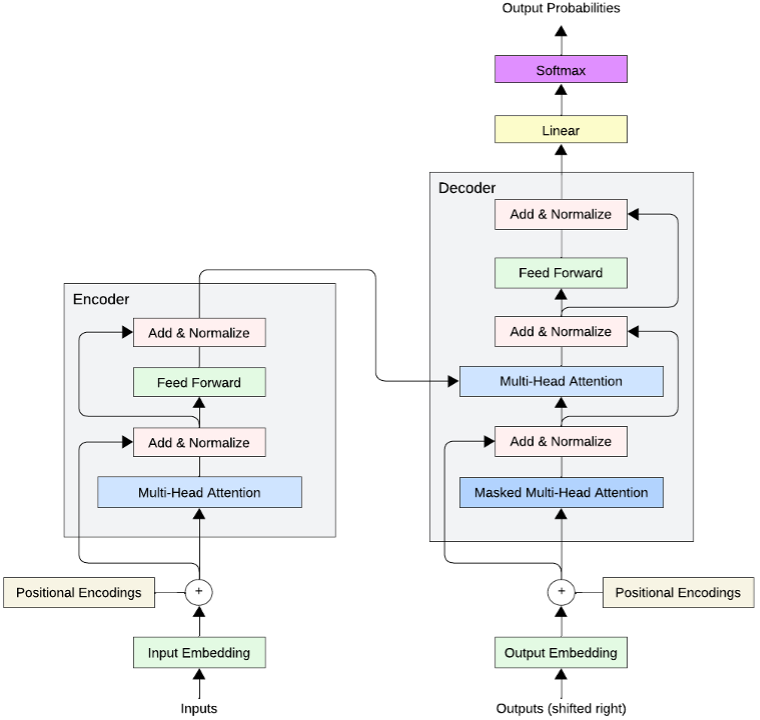
\includegraphics[width=1\linewidth]{images/transformers_architecture.png}
        \caption{The Transformer Architecture}
        \label{transformer}
\end{figure}

\subsection{Attention Mechanism}
This self-attention finds dependencies between all words in a text, short and long-term. The process of this starts by turning words into tokens. A token can be a word, subword, individual letter, or a sequence of words mapped to an embedding. The embedding is the vector representation of a token in high-dimension space; its size depends on how much information it stores about the token. Now, self-attention finds relationships between all tokens and gives them an attention score, measuring the relevance of a token to others. Transformers uses the scores to generate a final representation of each token. This process depends on how the models make a token. The tokenization strategy is determined by the preprocessing stage, and influenced by the embedding and model architecture. The embedding impacts the strategy because of its dimensionality, the amount of information encoded, and the model's sequence length limitations. 


\subsection{LLM Architecture}
In Figure \ref{transformer}, we can see an encoder and a decoder in the transformer architecture. Based on that, there are different LLM architectures: decoder-only, encoder-only, and encoder-decoder. Each one has advantages for specific tasks and limitations for others.


\begin{figure}[!hb]
    \centering
        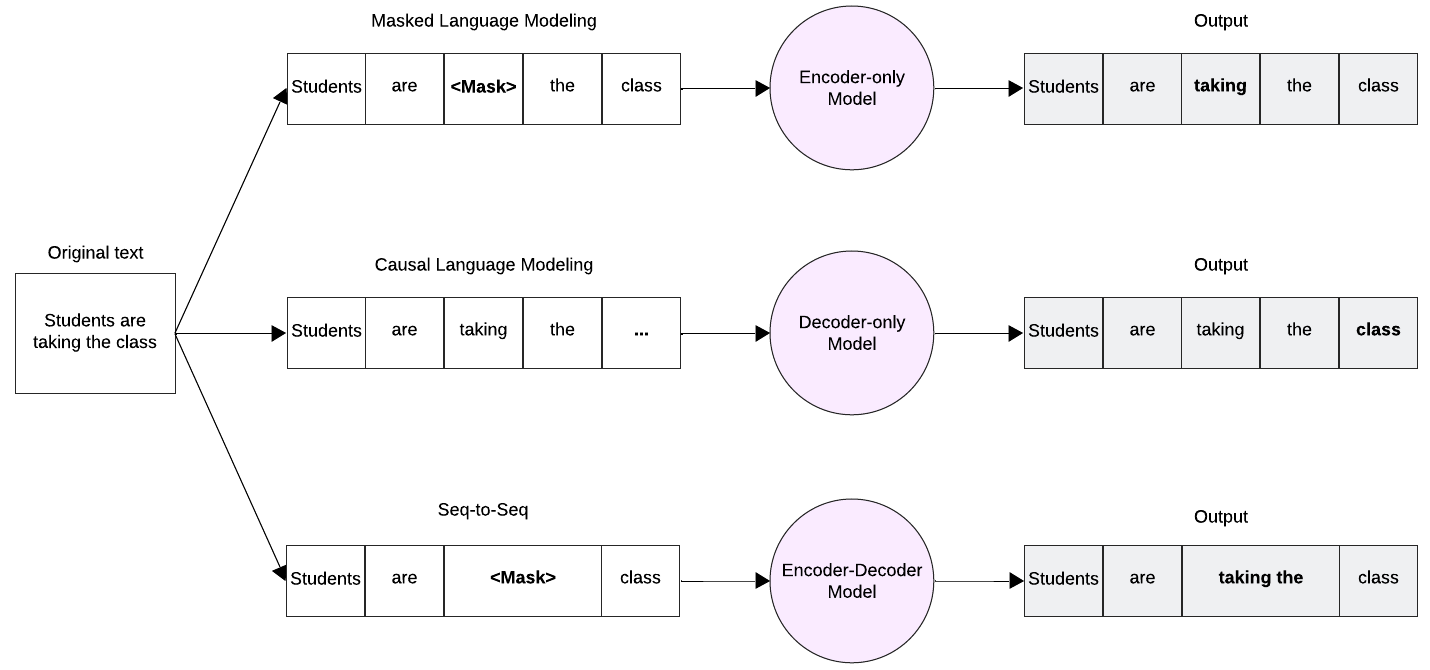
\includegraphics[width=1\linewidth]{images/LLM_Arch_text_generation.png}
        \caption{LLM Architecture and Comparison}
        \label{text_generation}
\end{figure}


\begin{description}

%\subsection{Decoder-only models}
\item[Decoder-only models:] Decoder-only models predict the next word based on the previous context, thus being unidirectional models. The model achieves this by taking a text or prompt as input and returning  a first word. For each subsequent word, the model uses the previously generated text as input to predict the next word, continuing until it produces a coherent output. In Figure \ref{text_generation}, the model predicts the last word based on the previous context. Because of their ability to predict sequences of texts, they are frequently employed in tasks like summarization and text generation. Models that perform those tasks are called causal language modeling (CLM) because they predict new tokens not found in the input. Compared to the other architectures, these models are massive in size. Because of their sizes, these are not very practical or cost-effective for daily usage. These are the most commonly known models, such as GPT-3 \cite{DBLP:journals/corr/abs-2005-14165}, Mistral \cite{jiang2023mistral7b}, and LLaMa \cite{touvron2023llamaopenefficientfoundation}.

%\subsection{Encoder-only models}
\item[Encoder-only models:] These models predict by masking specific words in a sentence. Said masking helps them understand the meaning or relation of the masked word based on context. They are bi-directional, which means they take the context before and after the masking to evaluate the word. The example in Figure \ref{text_generation} shows a sentence with a word mask being inputted to the encoder LLM. The model predicts the missing word by using the surrounding text. That is why they tend to perform well at classification and sentiment analysis but are not optimal for text generation. Said models are called masked language models (MLM). In contrast to other architectures, these models are relatively small. Some examples of encoder-only LLM are BERT \cite{DBLP:journals/corr/abs-1810-04805} and RoBERTa \cite{liu2019robertarobustlyoptimizedbert}.

%\subsection{Encoder-Decoder models}
\item[Encoder-Decoder models:] These models combine masking and text generation. They work by masking the sequence of texts and using the context around it to make a prediction. As seen in Figure \ref{text_generation}, they can mask more than one word from the original inputted text. Because the model generates sequences of texts, it is commonly used for translation and question and answer. Translating between languages cannot be achieved through word-for-word conversion; it requires understanding the entire sequence to preserve the context. To have an optimal model, both encoder and decoder must be trained for the task one wishes to achieve. Depending on the task, it can be harder to train compared to the other types of architectures. Bart \cite{lewis2019bartdenoisingsequencetosequencepretraining} and T5 \cite{2020t5} are examples of encoder-decoder LLMs.

\end{description}

Knowing the architectures, each one has its advantages for specific NLP tasks. However, to perform these tasks, we must train them to do so.


\subsection{Classification tasks}
Large Language Models use different learning methods to train. Such methods include zero-shot, one-shot, and few-shot learning. As the name implies, zero-shot learning is training a model without previous knowledge of the data; it is learning from scratch. One-shot learning is a method that receives one example as input and tries to generalize from that example. The final method uses multiple examples to find a pattern between them. 

In Figure \ref{gpt_example}, we can see an example of zero-shot learning. This LLM has no previous knowledge of the task that it must perform. Nonetheless, the model used, GPT-3, has the advantage that it can follow instructions when redacted clearly. Here, we tell the model that it must act as a medical expert and identify if a message is health-related and why it is classified that way.  Also, the result must follow a specific format. This process of instructions is called prompt engineering. Prompting does not retrain or adjust the model parameters. Thus, it does not always have optimal results.  
 
 \begin{figure}[!h]
    \centering
        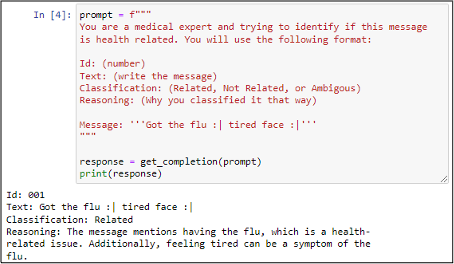
\includegraphics[width=0.9\linewidth]{images/gpt_example.png}
        \caption{Zero-shot example of GPT-3}
        \label{gpt_example}
\end{figure}


Moreover, LLMs that completed training with no additional modifications are known as based models. The response from this model will most likely make no sense with the premises it receives. This happens because the model is trained on excessive texts to find patterns between them, but this pattern might not be on par with the input. For the model to return a coherent response, it must go through a fine-tuning process. Fine-tuning consists of making a model perform specific tasks, such as chatting, summarization, chatbots, and others. To fine-tune a model, it must undergo another training process, with training data related to the tasks it will perform. However, there are multiple training types. We will focus on Sequence Classification and Causal Language Modeling.

\begin{itemize}
\item{\textbf{Sequence Classification:}} This involves predicting a class label based on an input. That label is a number associated with a class. All previously mentioned models can be trained for Sequence Classification, which is the most common training type.

\item{\textbf{Causal Language Modeling:}} This training is used for the model to learn the context of the text. We use this so the model learns to generate a text answer based on the input. The labels are texts related to the input. This type of training is similar to question-and-answer problems, in which the model infers a result based on the question. CLM is more expensive in computing power than Sequence Classification because  the labels must be embedded. That training type is most commonly used in models that have decoders because they are usually used to generate texts.

\end{itemize}

A problem with fine-tuning LLMs is that they require excessive computational resources to train or fine-tune. It is not viable to fine-tune all the parameters in the model to perform a specific task. However, there is an alternative to fine-tuning a model without having a resource problem.


\subsection{Low-Rank Adaptation (LoRA)}
The research in \cite{hu2021loralowrankadaptationlarge} created a technique to train models with billions of parameters effectively. Their technique, LoRA, helps reduce the amount of computational resources and
parameters to train while maintaining optimal performance. LoRA trains specific layers of the model instead of retraining the full system. Their research shows that they reduced the GPT-3 training size from 350GB to
35MB. However, a limitation of LoRA is that we must add the trained layer to the base model. That means that after training, we use both the base model and this adapted layer to perform a task. Nonetheless, it is still an
improvement when they reduced the resources used by a factor of 3x, and their model had an accuracy of \textpm 0.5\% compared to full fine-tuning. An effective fine-tuning process is possible, but we need to see some use
cases for these models.

\subsection{Example Applications}
The authors in \cite{koh2023groundinglanguagemodelsimages} trained a based LLM model to understand images and give a text description or a combination of text and image. The training process for
the model used images and their captions as their data and the zero-shot learning strategy. Their resulting model was used as a chatbot that identifies images, answers questions, or gives
visual examples. Another experiment was \cite{inproceedings}, where the authors trained a model to identify sentiments on financial market decisions. In this case, they used prompting, also called in-context learning, for 
the model to answer the sentiment of the texts. In-context learning does not update any parameter of the original model. Their model resulted in a 70\% accuracy on sentiment prediction, failing mostly on neutral posts.
A possible problem with the neutral post is that prompting does not train the model to perform a specific task. That experiment showed the problem that users face when they use social media to make decisions.
They clarified the importance of not taking the model for granted and how social media can cause a user to make a poor decision.

\subsection{Challenges and Limitations}
An issue with LLM is that they answer based on statistical relationships between words, and occasionally, their output could make no sense. Sometimes, they can generate a result that is not factual
or valid; this phenomenon is called AI hallucinations. These models train to find patterns between tokens. Without the proper context, they cannot differentiate between fact and fallacy. This context
needs to  be related or similar to the input that the model receives. However, finding the necessary information is not optimal if done manually. That begs the question, how much data would be needed
to achieve a coherent answer, and how can this be done effectively?


\section{Vector Databases}
AI hallucinations occur when models generate a plausible output but lack factual accuracy. We can minimize the hallucinations by providing context relating to the text inputted. A solution to this
is finding data from officials or experts on the topic associated with the text. Given the vast amount of research available, narrowing down relevant information becomes a challenge. In addition,
the context quality is essential for the model to make any inference. The search process for this consumes time and is not always optimal. 

Nonetheless, if we have an immense amount of data from different sources, we can benefit by using a vector database. In contrast to other databases, they store data in a vector representation.
These databases can come in different forms, like Chroma \cite{chroma}, a native vector database. Also, some relational databases have extensions that allow them to make vector similarity searches,
like Postgres with pgvector \cite{pgvector}. They can turn images, videos, documents, and others into numerical embedding. These embeddings are numerical vectors capturing semantic meaning \cite{10455990}.
They are practical because the system stores the data provided as vectors in a high-dimensional space, where semantically similar data are positioned close in said space. We can see a text example of the vector
space in \ref{vector_space}. If we search for ``Flu" it should return ``Sick" or ``Covid" with a higher probability than ``Car" or ``Truck". As we can see, querying this database will return a result close to the input.

  \begin{figure}[!h]
    \centering
        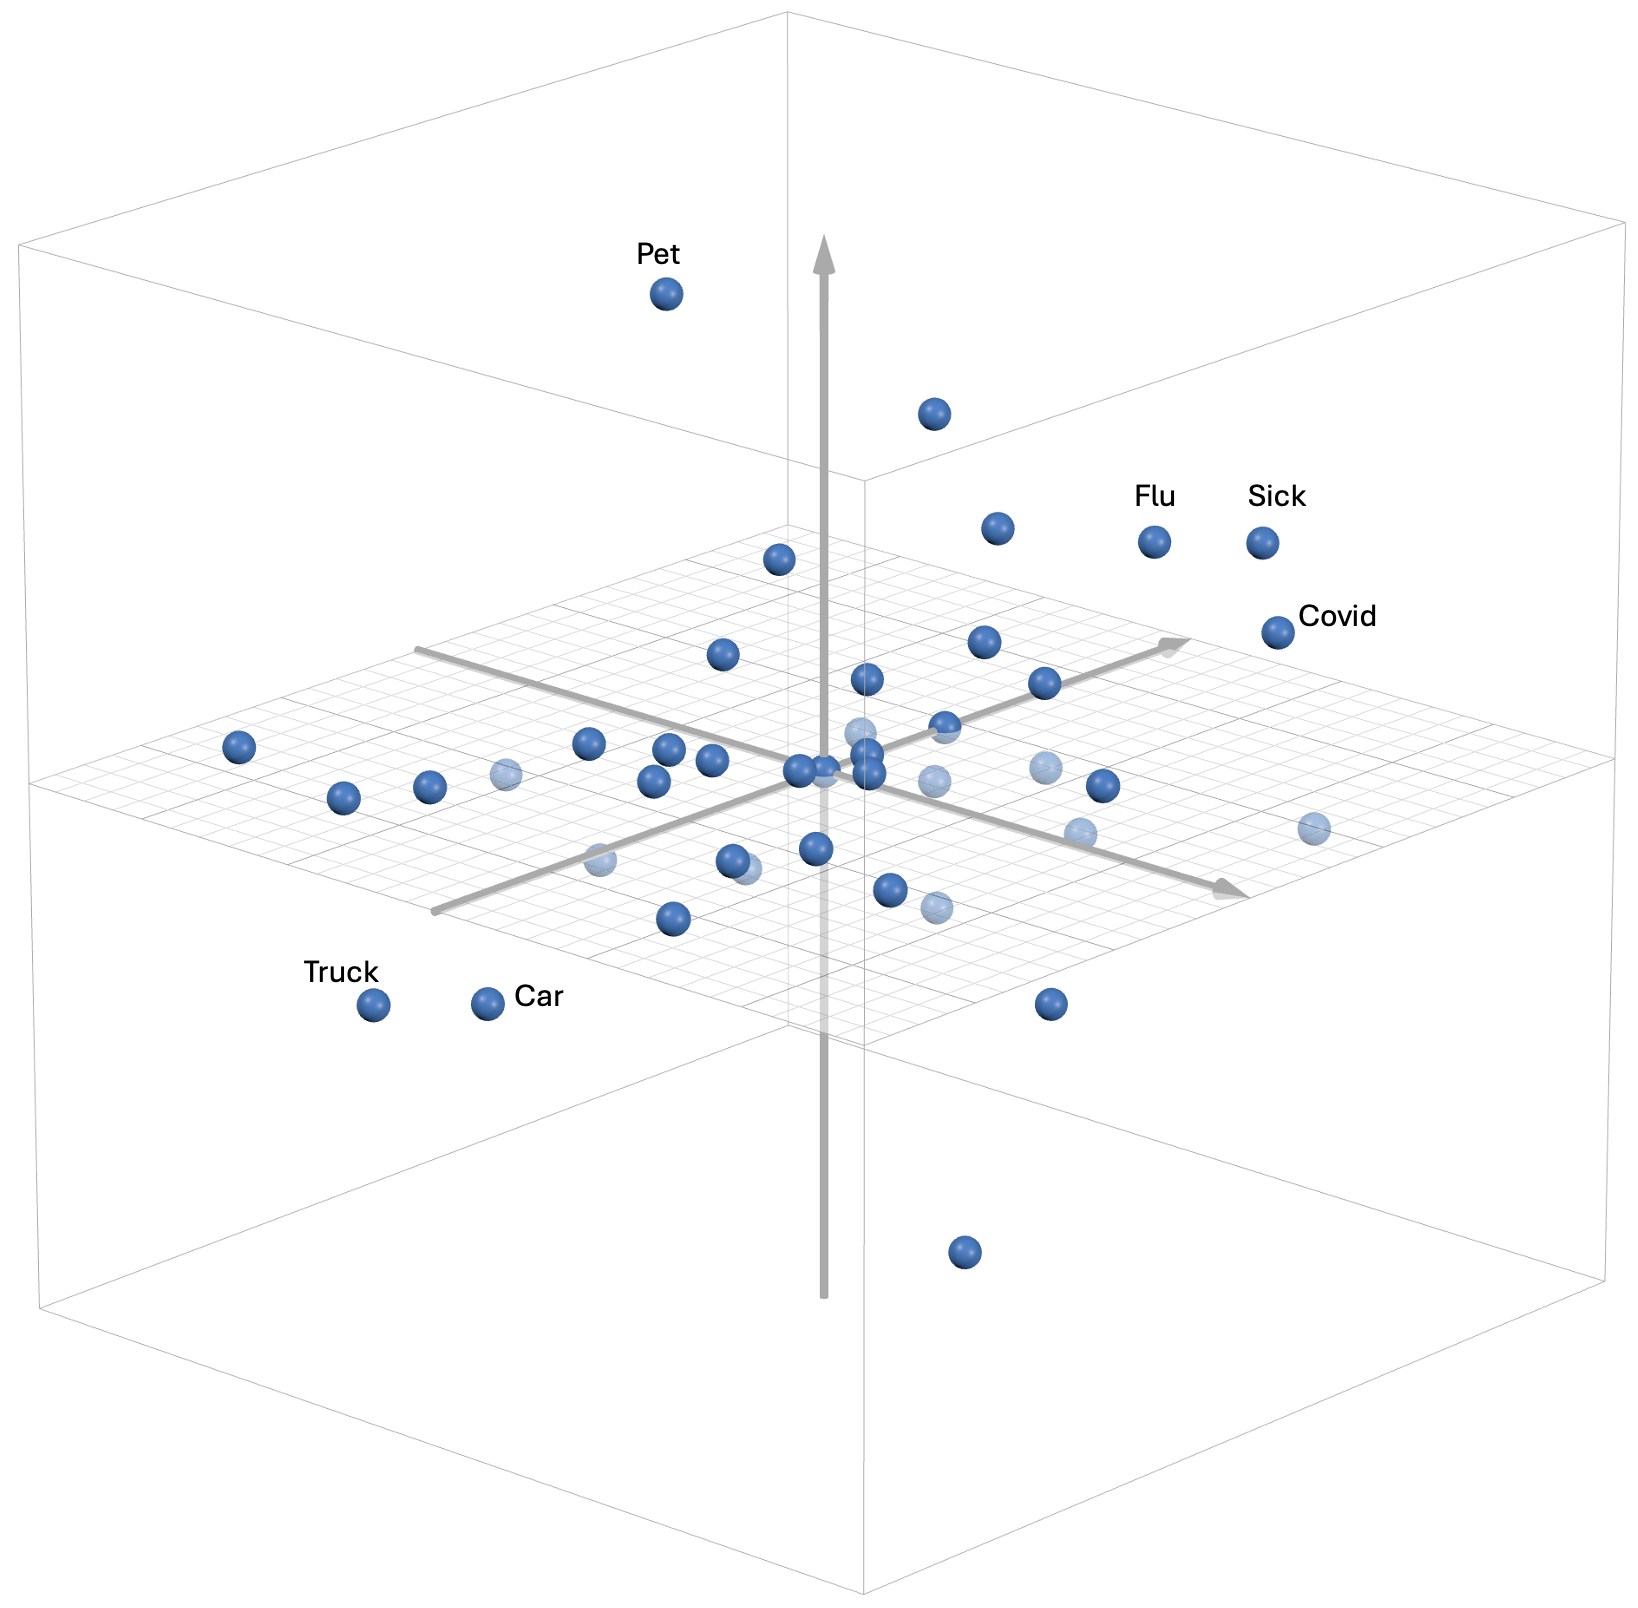
\includegraphics[width=0.85\linewidth]{images/Vector_example_update.png}
        \caption{High-Dimensional Space Representation}
        \label{vector_space}
\end{figure}

Although these systems help find similar text, there are a few limitations. One such problem is the vector size, which can impact the accuracy and resource usage \cite{han2023comprehensivesurveyvectordatabase}. If
the vector size is relatively big, the system will have a higher accuracy but will require more storage and resources to process. Also, this affects when searching large datasets, which incurs a resource-intensive search.
 
For the data insertion process, we need to find optimal strategies for our data. If we focus on a text dataset, the best practice is to split the document into chunks. This splitting process must be optimal for the task we want
to achieve. If we split it into small chunks, it will have a more precise answer, but we dilute the meaning of the text. On the other hand, larger chunks can have more context but less relevance. After selecting the appropriate
size, these chunks must be turned into a vector, usually done with an LLM. Finally, we store these vectors and their chunks in the database system. 

To search the system, we send a query to the LLM that converts it into a vector. Then, the vector is used in the database to make a similarity search. The system will return chunks that can function as context for an LLM to
analyze. In this context, an LLM can use the retrieved chunks to generate a fact-based answer from outside their initial training. This process, known as Retrieval-Augmented Generation (RAG), enables LLMs to access relevant
information during text generation. In \cite{10683437} they tested LLM to answer a test that contained images and text. They evaluate the GPT3 base model, the base model with prompt, and a GPT3 with RAG. Their experiments
showed that the base model's average success ratio was 40\%, the second model was 58\%, and the model with RAG ended with 75\%. Said experiment showed that an LLM can have excellent performance when it receives the necessary context.
Therefore, RAG can assist in providing expert-level responses, but human oversight is still imperative for complex topics. Additionally, in a world with many sources of information that can be misleading to people, this can help identify
texts that are not factual or incorrect. 


\section{Misinformation in Social Media}
There are many sources in the world to find information about any topic. Nonetheless, many people use social media as their primary source \cite{socialmedias} and occasionally take this information as truth without
validation \cite{social_fact}. On occasion, these can be fake, misleading, or wrong. When this happens unintentionally or by lack of understanding of the topic, it is called misinformation. On the other hand,
when it is intentional to provide wrong information, this is known as disinformation. For simplification, both terms will be used interchangeably, as they have a similar impact on the user and give information that is not accurate.

Misinformation has been dangerous during critical events like natural disasters or health crises. For instance, during the COVID-19 pandemic, false claims appeared saying that the vaccine had
microchips or that it was intended for population control \cite{article_vaccine}, which led to high health risks or even deaths \cite{article} because people refused to get vaccinated out of fear. A problem with disinformation is that the audience
does not always detect it. When misinformation spreads and is not clarified early on, it can be confused as fact. Misinformation can affect all demographics, but older audiences and people with less education are more
likely to share and believe fake or misleading news  \cite{encyclopedia3040099}. 

There have been various research studies on reducing the propagation of misinformation. Misinformation was modeled as a game-theoretic problem in \cite{9906925}, where some players spread fake news, and others tried
to stop it. They created an agent at the network level to combat misinformation in a simulation. However, they could not conclude the efficiency of their model due to the lack of discernible patterns in the simulation. On
the other hand, the authors in \cite{10100054} used LSTM and BERT to classify misinformation from the different news sources. They showed that BERT outperformed LSTM, achieving an accuracy of 64.88\% against 60.59\%. 
These results are significant in detecting misinformation; still, they are not optimal for situations that can directly impact someone's life. For example, the system has over a third chance of misclassifying news, and this could
be dangerous if the topic is a natural disaster or health risk. We need to ensure that AI models classify this type of news with a very high accuracy rate. 

Another approach to detecting fake information was on \cite{Ayoobi_2023}, where they detected fake LinkedIn profiles. On this occasion, the dataset used for training included real and AI-generated profiles. They tested multiple
LLMs like BERT and RoBERTa, but BERT resulted in the highest accuracy of 95.67\%. These investigations showed the efficiency of Large Language Models for Natural Language Processing in the misinformation field. Regardless,
none of these studies addresses health-related misinformation on social media. 

When combatting misinformation, the difficulty arises when determining what is spreading and how experts can correct it. To determine if a text is spreading lies, one must understand or find credible sources,
such as peer-reviewed studies or expert opinions, to verify the truth. Some disinformation can be easier to identify such as hoaxes, but other things, such as conspiracy theories, require more resources to debunk.
When the topic of the text becomes complex or not identifiable, some credible sources help with the rebuttal. These tasks are time-consuming and require an expert in the field for accuracy. In addition, the
explanation must be expressed so that any audience can understand it. These are a few reasons that health-related misinformation is hard to combat. It requires professionals in the field to be fast at identifying
misinformation and concise when correcting them. With the advancement in Artificial Intelligence, LLM can combat misinformation by classifying it and rebutting it. For the classification process, it is possible to
finetune an LLM that determines if a text is misinformation. Additionally, it can generate rebuttals using RAG. With a vector database that contains peer-reviewed research, it can ensure that the information is factual. 
This AI approach can reduce the dependency on experts and have a system that can act in real-time to prevent a significant spread of misinformation.


\section{Twitter Health Surveillance (THS)}
The THS system classified tweets related to health issues \cite{8622504}. The system utilized LSTM and GRU to classify tweets as being medical related, medical unrelated, or ambiguous.  The THS
data extraction pipeline can be found on Figure \ref{ths_architecture}. First they extracted data from the Twitter API and sent that data to an Apache Kafka queue. Then, a consumer sent it to Apache Spark
to process the data and store it in a Hive warehouse. Later, a preprocessing phase for each tweet occurred, which removed hashtags, mentions, emojis, and web links. The classification agent trained with the resulting
plain text. This version used recurrent neural network (RNN) and 1-d convolutional networks because of their advantages with sequential data. They tested various combination architectures, but the one with the highest result was an
LSTM layer, with no attention, and a GRU layer; it had an F1 score of 86\%, a recall of 89\%, and a precision of 83\%.  
 
  \begin{figure}[!h]
    \centering
        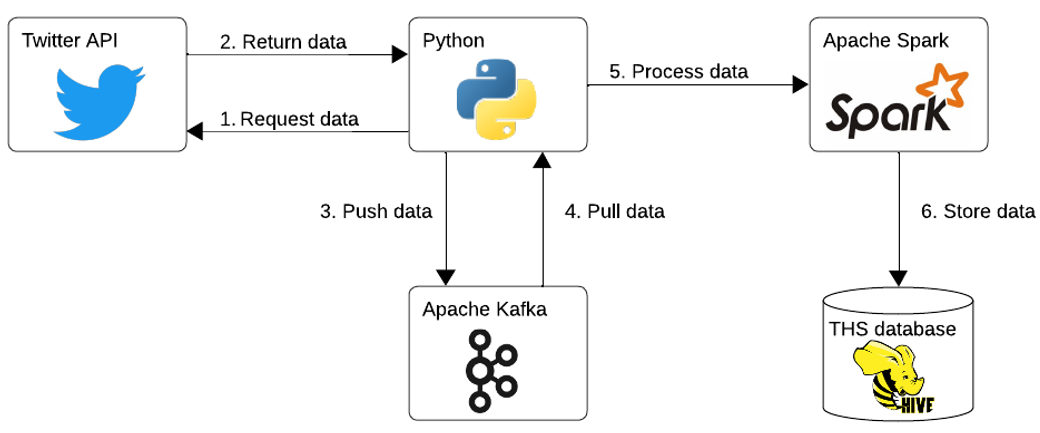
\includegraphics[width=1\linewidth]{images/ths_architecture.png}
        \caption{THS Architecture}
        \label{ths_architecture}
\end{figure}

 
Later the project was updated to find similarities between tweets \cite{9581175}. This new version tested convolutional neural networks (CNN) and recurrent neural networks to classify how closely related are two different tweets.
They used a ranking method that gave a higher score if two randomly selected tweets were similar. The agent received an input of triplets where the first element was compared against the other two elements.
The system trained on two data types: raw tweets and cleaned tweets. This latter had stop-words removed and a lemmatization process. Cleaned tweets proved a higher accuracy in the recurrent neural network
for regular LSTM and bidirectional networks; in contrast, the raw tweet had a better result in CNN validation. All three models had similar results; the highest validation accuracy was the regular LSTM with 90\%,
followed by the other two with 87\%. Nonetheless, the training time for the CNN was the fastest, with regular LSTM in second place and the slowest being the bidirectional LSTM network. 


  \begin{figure}[!h]
    \centering
        
\includegraphics[width=0.8\linewidth]{images/base_gpt_health.png}
        \caption{ChatGPT Classification Example – Health Related}
        \label{gpt_health}
\end{figure}

However, both of these experiments removed special characters or elements from the original text. By then, tweets had a limitation of characters, making each one of the crucial the context. Removing special
characters, could remove information that the author of the text intended. We can have the example in Figure \ref{gpt_health}, where a base GPT model  classified a text. The model uses the hashtag and mention
as context to determine if the text is health related or not. This is a good presumption, but these platforms' users could use hashtags or mentions that are not relevant to the text. 




% Define a custom style for JSON formatting
\lstdefinelanguage{json}{
    basicstyle=\ttfamily\small,
    numbers=left,
    numberstyle=\tiny\color{gray},
    stepnumber=1,
    numbersep=8pt,
    showstringspaces=false,
    breaklines=true,
    frame=single,
    backgroundcolor=\color{gray!10},
    keywordstyle=\color{blue},
    stringstyle=\color{red},
    morestring=[b]",
    morecomment=[l]{:}
}




\chapter{System Architecture}  

\section{Paper ETL Pipeline}

Our model must use credible sources of information to rebut misinformation. We identified PubMed \cite{pubmed}, an online library that contains peer-reviewed medical literature. We want to extract the papers and store them in a vector database. To extract these papers, we used the BioC API \cite{bioinformatics}, which has access to the PubMed library. However, the API needs the research paper's identifier, known as PubMed Central (PMC) ID. We design a scraper to extract these identifiers from the official PubMed site. The pipeline in Figure \ref{fig:etl} shows the processes of data extraction. 

\begin{figure}[H]
	\begin{center}
		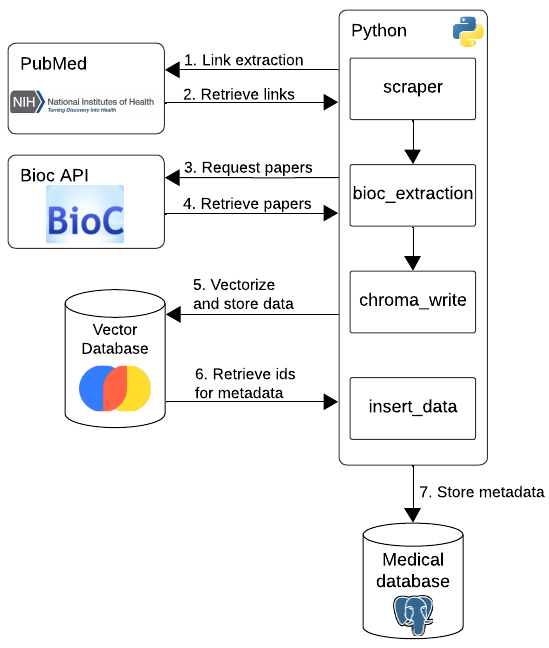
\includegraphics[width=0.75\textwidth]{images/ETL_Pipeline.png} %specify width
	\end{center}
	\caption{Medical Data Extraction Pipeline} %specify caption
	\label{fig:etl}
\end{figure}

\subsection{Scraper}
The first step of the pipeline was identifying what papers we needed to extract. We selected 17 topics for the data extraction process, that can be seen in Table \ref{table:topics}.

\begin{table}[!ht]
	\centering
	\caption{Topics for Research Paper Extraction}
	\begin{tabular}{||c | c||} 
			\hline
			 \multicolumn{2}{||c||}{\textbf{Topics}} \\ [1.5ex] 
			\hline
			allergy  & covid vaccine \\ [1ex]
			\hline
			bird flu & flu vaccine \\ [1ex]
			\hline
			cancer & headache \\ [1ex]
			\hline
			chickenpox & influenza\\ [1ex]
			\hline
			common cold & monkeypox \\ [1ex]
			\hline
			conjunctivitis & stomach aches \\ [1ex]
			\hline
			covid sickness & swine flu \\ [1ex]
			\hline
			covid symptoms & zika\\ [1ex]
			\hline
			covid treatment &  \\ [1ex]
			\hline
			\end{tabular}
	\label{table:topics}
\end{table}


To extract them, we built a scraper in Python using Selenium and BeautifulSoup libraries. We used Selenium to retrieve the web source from PubMed's website, and BeautifulSoup was used to get the links to each paper. These links contained the PMC identifier. For each topic, we selected 5,000 PMC identifiers. These identifiers were grouped by topic and stored locally in Comma Separated Value (CSV) files.

\subsection{BioC API}
After retrieving those identifiers, we need to extract the research papers. Using the PubMed API, BioC, we made requests that returned the documents as JSON. These JSONs were preprocessed to contain texts, and we removed tables and figures. Later, the paper's sections -introduction, methodology, results, and others- were combined as one attribute, excluding references. We removed tables, figures, and references from the context to ensure the chunking process worked appropriately. If the data is not preprocessed, when performing RAG, we can retrieve data that is not useful. After that, we turned the result into a new JSON that contained the research metadata and its context. 

\subsection{Vectorizing data}
Later, each research paper’s context was split into chunks using LangChain. Then, we used an LLM, BAAI \cite{bge_embedding}, to embed these chunks. A universal unique identifier (UUID) was combined with each chunk and stored in a Chroma \cite{chroma} database. After uploading the data to Chroma, we added these UUIDs to their JSON. 


\subsection{Store metadata}
Now, with all papers vectorized, we upload the metadata into a Postgres database. First, we validate that there are no duplicate records in the system. To prevent duplicates, we search for the paper's reference. If any is found, we delete the chunks from the vector database. Additionally, any research that did not contain at least an abstract was removed. That ensures that there is no repetition or inconsistency when doing the rebuttal. Later, we upload this data into the system following the schema found in Figure \ref{fig:table}. The tables in this schema are as follow:

\begin{description}
	\item{\textbf{Research:}}  The table contains the research paper data. Its attributes are title, which is the research paper title; context, the paper’s text; paper\_ref, the complete reference of the paper, used to prevent duplicates; and fullpaper, which is a boolean that is true if the paper contains an abstract, introduction, methodology, discussion, conclusion, and references.
	\item{\textbf{Chunks:}} This table pairs the UUIDs from the paper's chunks and their respective research record.  
	\item{\textbf{Keyword:}} Some research papers contain keywords that allow the reader to know the subjects mentioned in the paper. 
	\item{\textbf{Author:}} Stores the first and last names of all authors identified in the research paper. 
	\item{\textbf{Reference:}} All references that are present in the research paper.
	\item{\textbf{Topic:}} This contains the different topics used to search the papers.

\end{description}

\begin{figure}[H]
	\begin{center}
		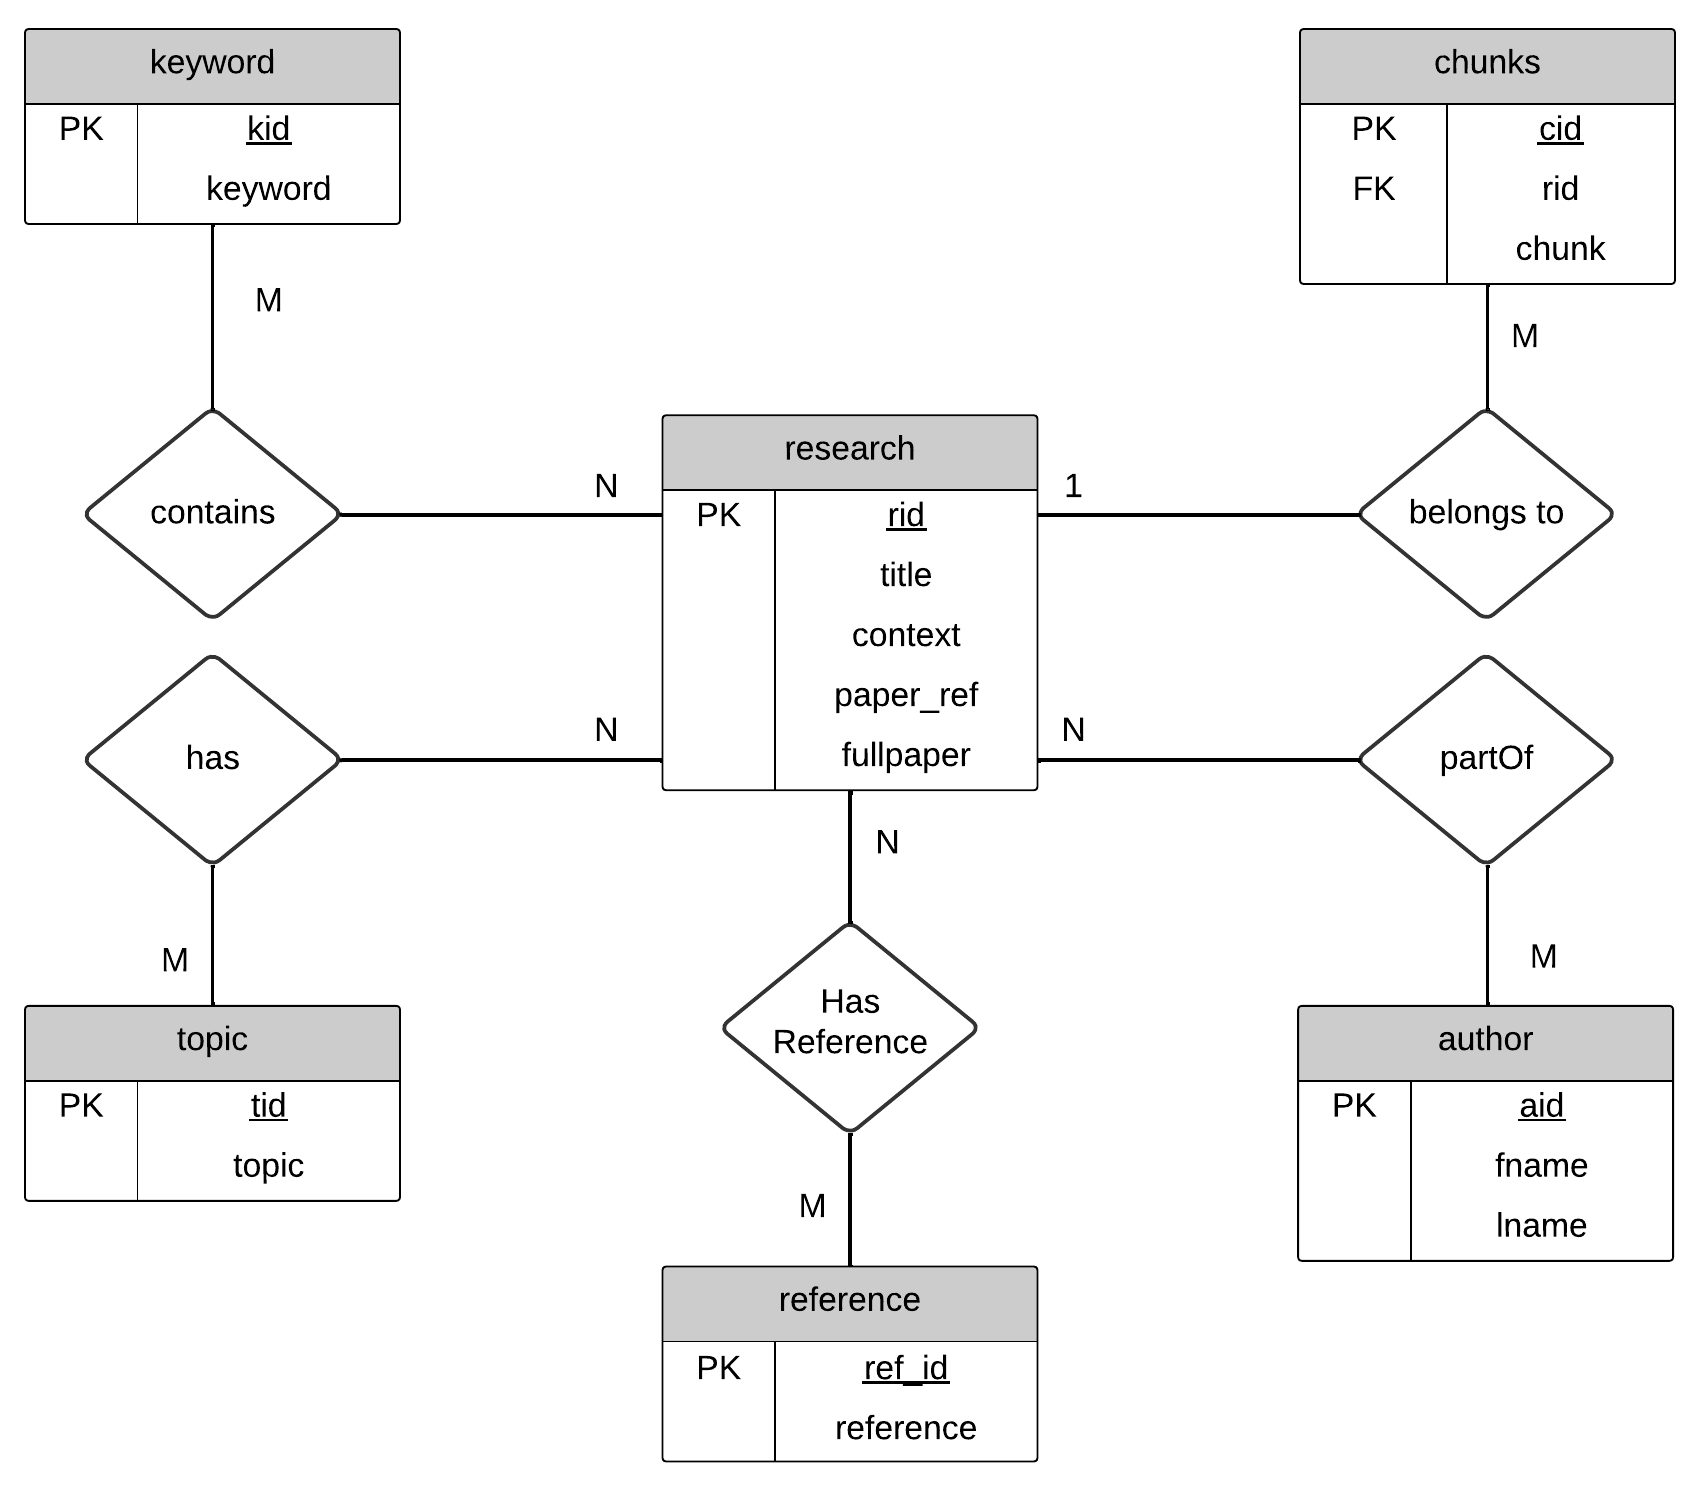
\includegraphics[width=0.9\textwidth]{images/Table_diagram.png} %specify width
	\end{center}
	\caption{Research Papers Schema Diagram} %specify caption
	\label{fig:table}
\end{figure}


We started the search with 85,000 peer-reviewed papers. After finishing the filtering and data cleaning, we ended with 56,365 different research papers. 



\section{Misinformation Rebuttal Pipeline}
After training the models and storing the context for the rebuttal, we create the model pipeline. The pipeline shown in Figure \ref{fig:llm} shows the process of receiving a text, making the classifications, and returning an explanation of why it is misinformation.

\begin{figure}[H]
	\begin{center}
		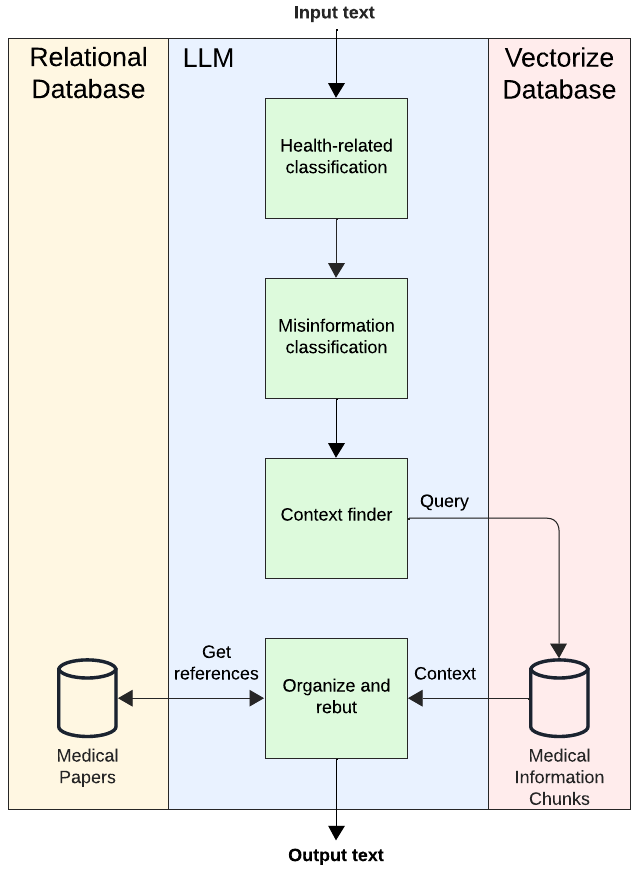
\includegraphics[width=0.75\textwidth]{images/LLM_Pipeline} %specify width
	\end{center}
	\caption{Misinformation Rebuttal LLM System Architecture} %specify caption
	\label{fig:llm}
\end{figure}


\subsection{Health-related Classification}
The first part of the pipeline is determining if the text is related to health. When the system receives the input text, it sends it to a model finetuned to classify health-related texts. This model determines whether the input is related, unrelated, or ambiguous.
If the text is health-related, we continue to the next part of the pipeline. When the text is non-related or ambiguous, we end the process. We end this because other topics are out of the model's scope. 

\subsection{Misinformation Classification}
After confirming that the text is health-related, we want to validate that it contains misinformation. The finetuned model can only return two possible results: misinformation or non-misinformation. If the model finds no misinformation after evaluating the text,
the final output will return both classifications. When the result contains misinformation, we start the search for research papers.

\subsection{Context Finder}
Before starting the search on the vector database, we must understand the topic of the text. To automate this process and generate a query as precise as possible, we use Ollama \cite{ollama}. That tool allows us to execute locally a pre-trained LLM that generates text. Thus, we send a query to Ollama asking it to make a one-sentence query for the vector database related to the input.

 
 \begin{tcolorbox}[colback=gray!10, colframe=black!70, title=Input]
\texttt{%
\#nih fauci, @cdcdirector @sgottliebfda \&amp; @barda bright expected to be grilled tomorrow over ineffective \#flu vaccine at @housecommerce \#suboversight bets on fauci saying universal \#influenza vax in 5, maybe 10 years? my preview here: \url{https://t.co/fsqefwhik7} \#cdc \#fda \#vaccines%
}
\end{tcolorbox}

\begin{tcolorbox}[colback=white, colframe=black!70, title=Output]
\textit{%
Flu vaccine effectiveness and future universal influenza vaccination strategies.%
}
\end{tcolorbox}
 
The above example shows that Ollama can identify the topics of the original text. That tweet mentions that the flu vaccine is ineffective and asks how long it will take for a universal influenza vaccine. The LLM identified the topic and made a query that can help find
research papers related to it. However, it is essential to mention that the LLM output can vary. As mentioned previously, this is a statistical model and can have slight variations in its result. Now, this output is sent to the Chroma database to retrieve chunks of research
papers. For this experiment, our model returns eight chunks that are closest in context to the query. These chunks are then sent to another model to be analyzed and organized.

\subsection{Organize and Rebut}
The final part of our pipeline is using RAG to provide an answer that explains why the original text is misinformation. First, we retrieve the references of the chunks we use for the context. Then, we send the original text with the chunks, as context, to Ollama for
the model to evaluate. Ollama returns a 2-3 sentence result that explains the text’s misinformation. The final output is a JSON with the following attributes:

\begin{description}
\item{\textbf{chroma\_value:}} If the text is health-related and is misinformation, this will have the rebuttal output from Ollama, consisting of 2-3 sentences. If the text is non-related or non-misinformation, it will give a default value saying so. 
\item{\textbf{health:}} This is the input text health classification.
\item{\textbf{misinformation:}} This is the input text misinformation classification.
\item{\textbf{references:}} This attribute stores the list of references used for the rebuttal. 
\item{\textbf{t\_context:}} The original text.

\end{description}

The pipeline enables us to automate the classification process and rebut misinformation using peer-reviewed research. By leveraging fine-tuned models, vector search, and RAG, the architecture provides concise, fact-based responses. A key advantage of this
approach is its ability to explain complex content accessible to non-technical readers, giving them a clearer understanding of false information. This can assist professionals in the field to mitigate the spread of lies that can negatively impact public health.


\section{User Interface (UI)}
With the pipeline correctly working, users need to interact and view the results. We created an user interface were they can interact with texts and see the classification process. Figure \ref{fig:Menu} shows the main menu of the interface. When we select a text a side screen appears that shows the results from the misinformation classification pipeline. 

\begin{figure}[!ht]
\noindent\makebox[\textwidth][l] {%
	\hspace{-\dimexpr\oddsidemargin} % -\dimexpr\oddsidemargin+0.1\paperwidth -> x * 0.5 - 0.375
		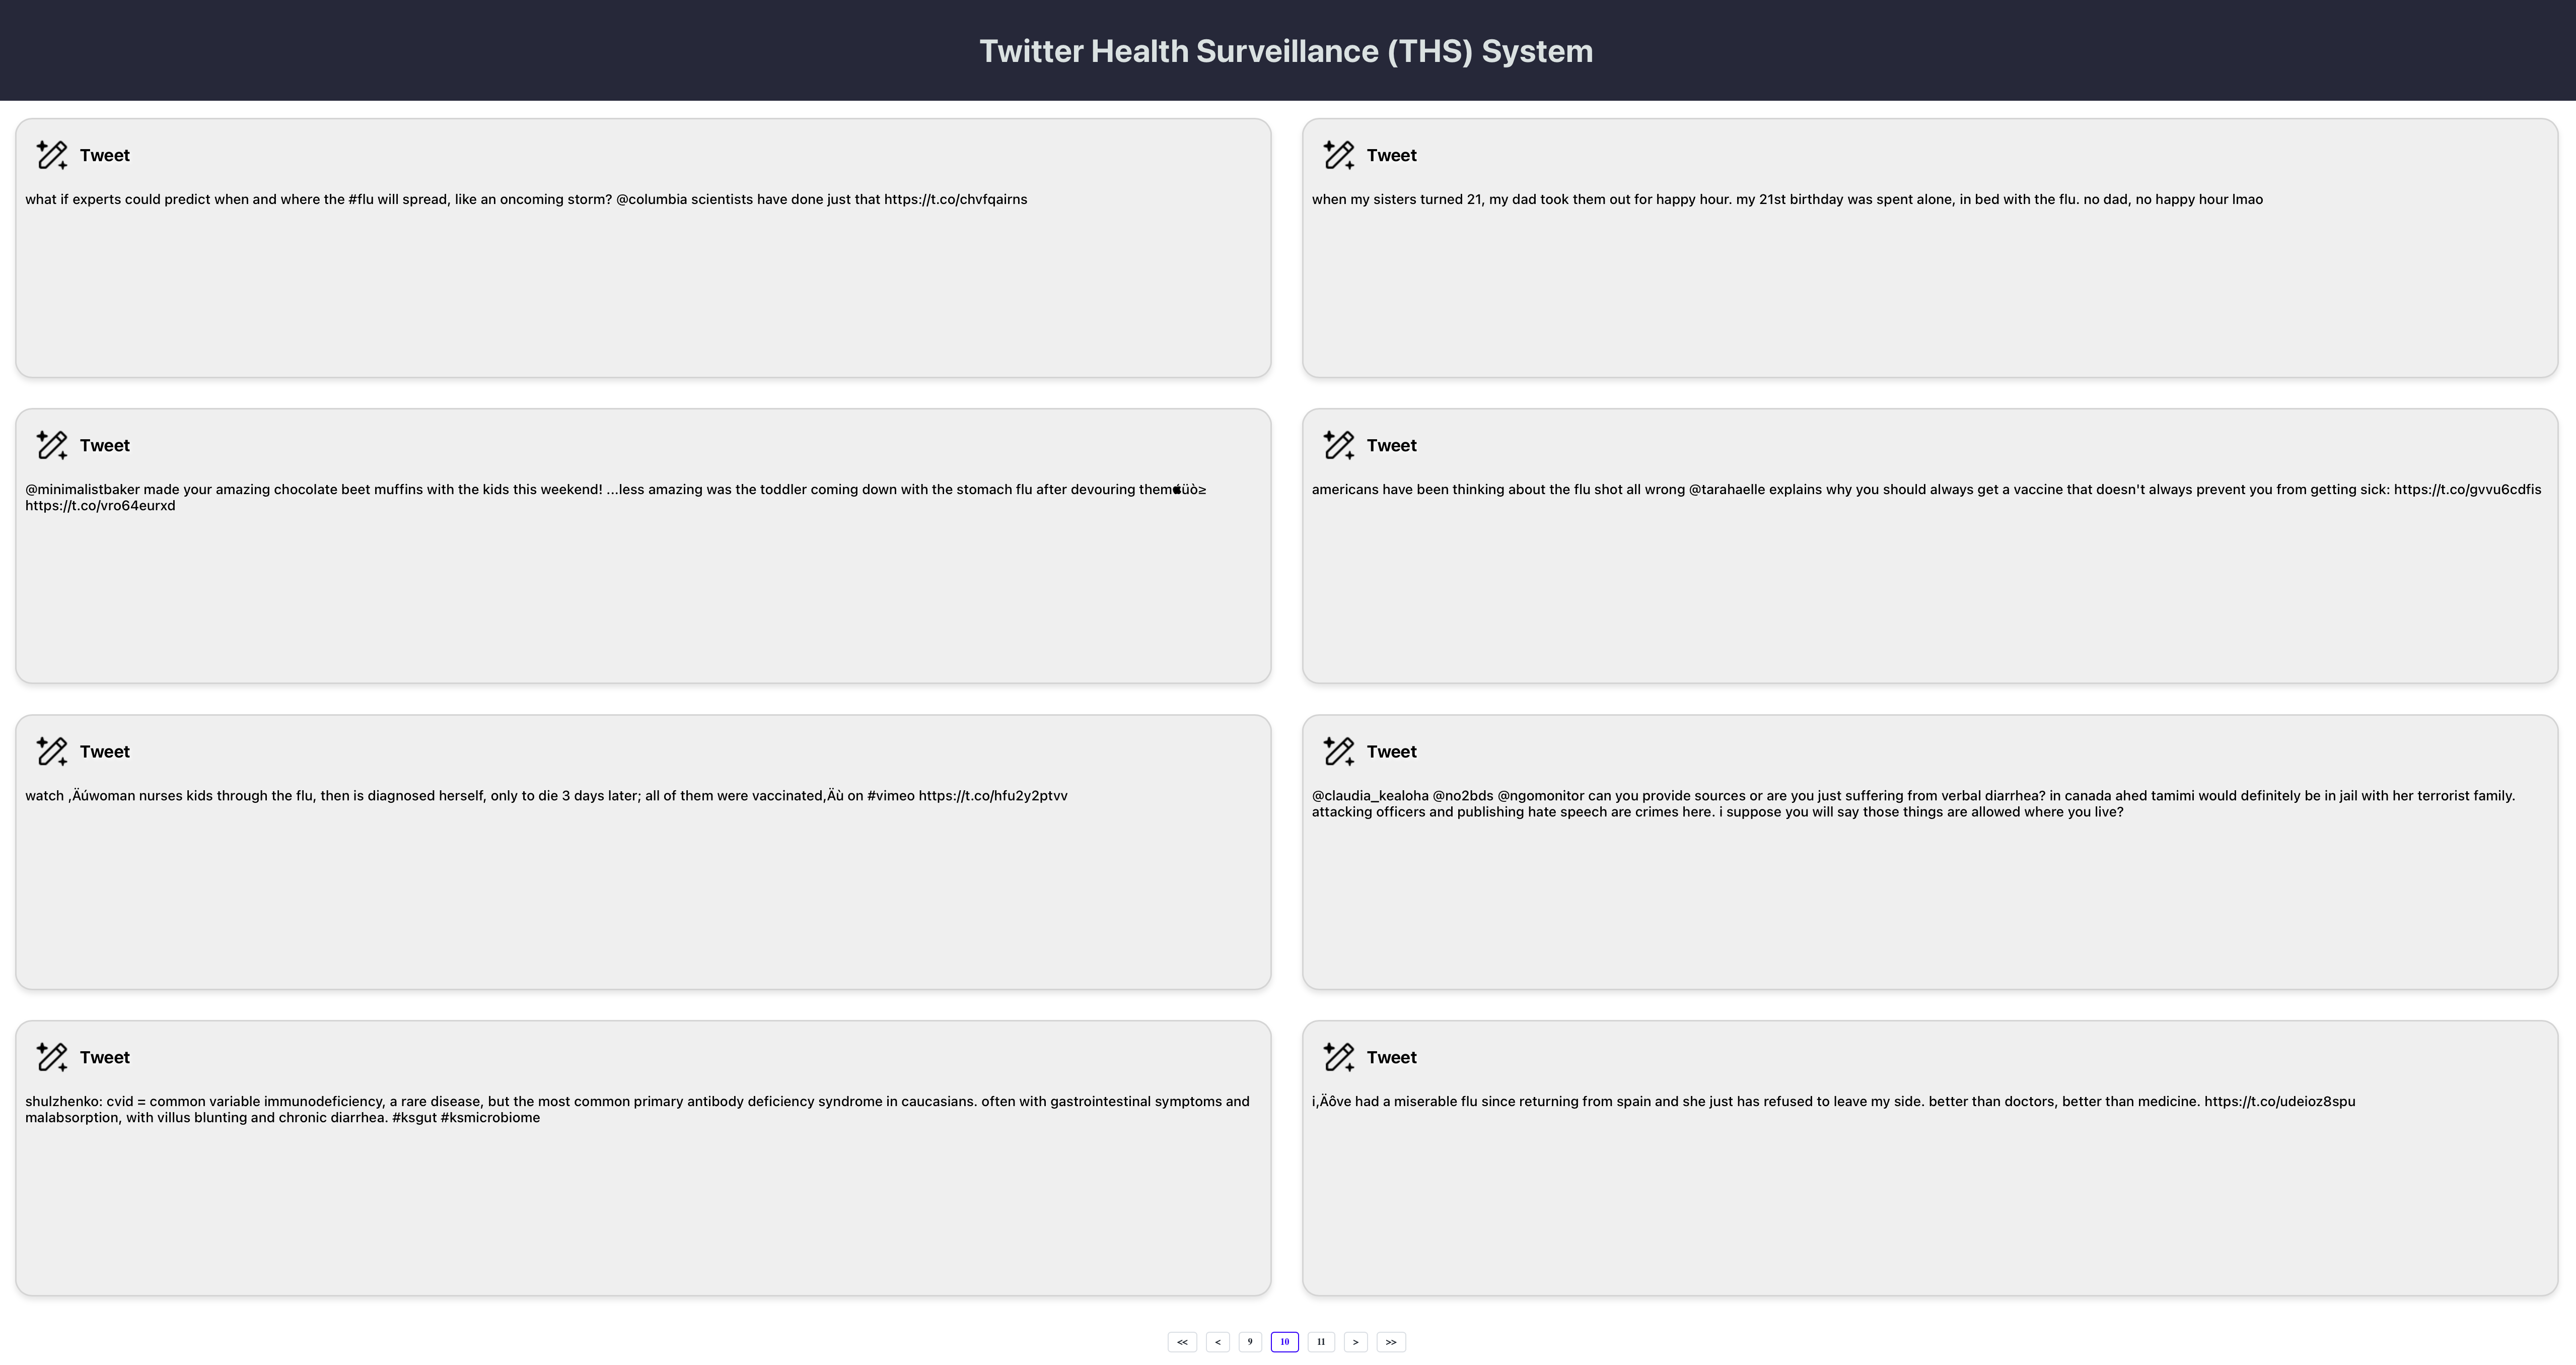
\includegraphics[width=0.75\paperwidth]{images/THS_Frontend_Menu.png} %specify width
	}%
	\caption{THS Frontend - Menu} %specify caption
	\label{fig:Menu}
\end{figure}

Figure \ref{fig:frontendmisinformation}  presents a case where the models classified the text as health-related and misinformation. The top of the side screen shows the text that was classified. Number 1 shows the health classification, and number 2 shows the misinformation classification. Below that is the rebuttal generated by the models. Finally, we include the references of the research used for the rebuttal. An alternative view of the side screen is Figure \ref{fig:frontendnonmisinformation}; when it does not find misinformation, the model does not generate an answer nor cite any research.

\begin{figure}[H]
\noindent\makebox[\textwidth][l] {%
	\hspace{-\dimexpr\oddsidemargin}
		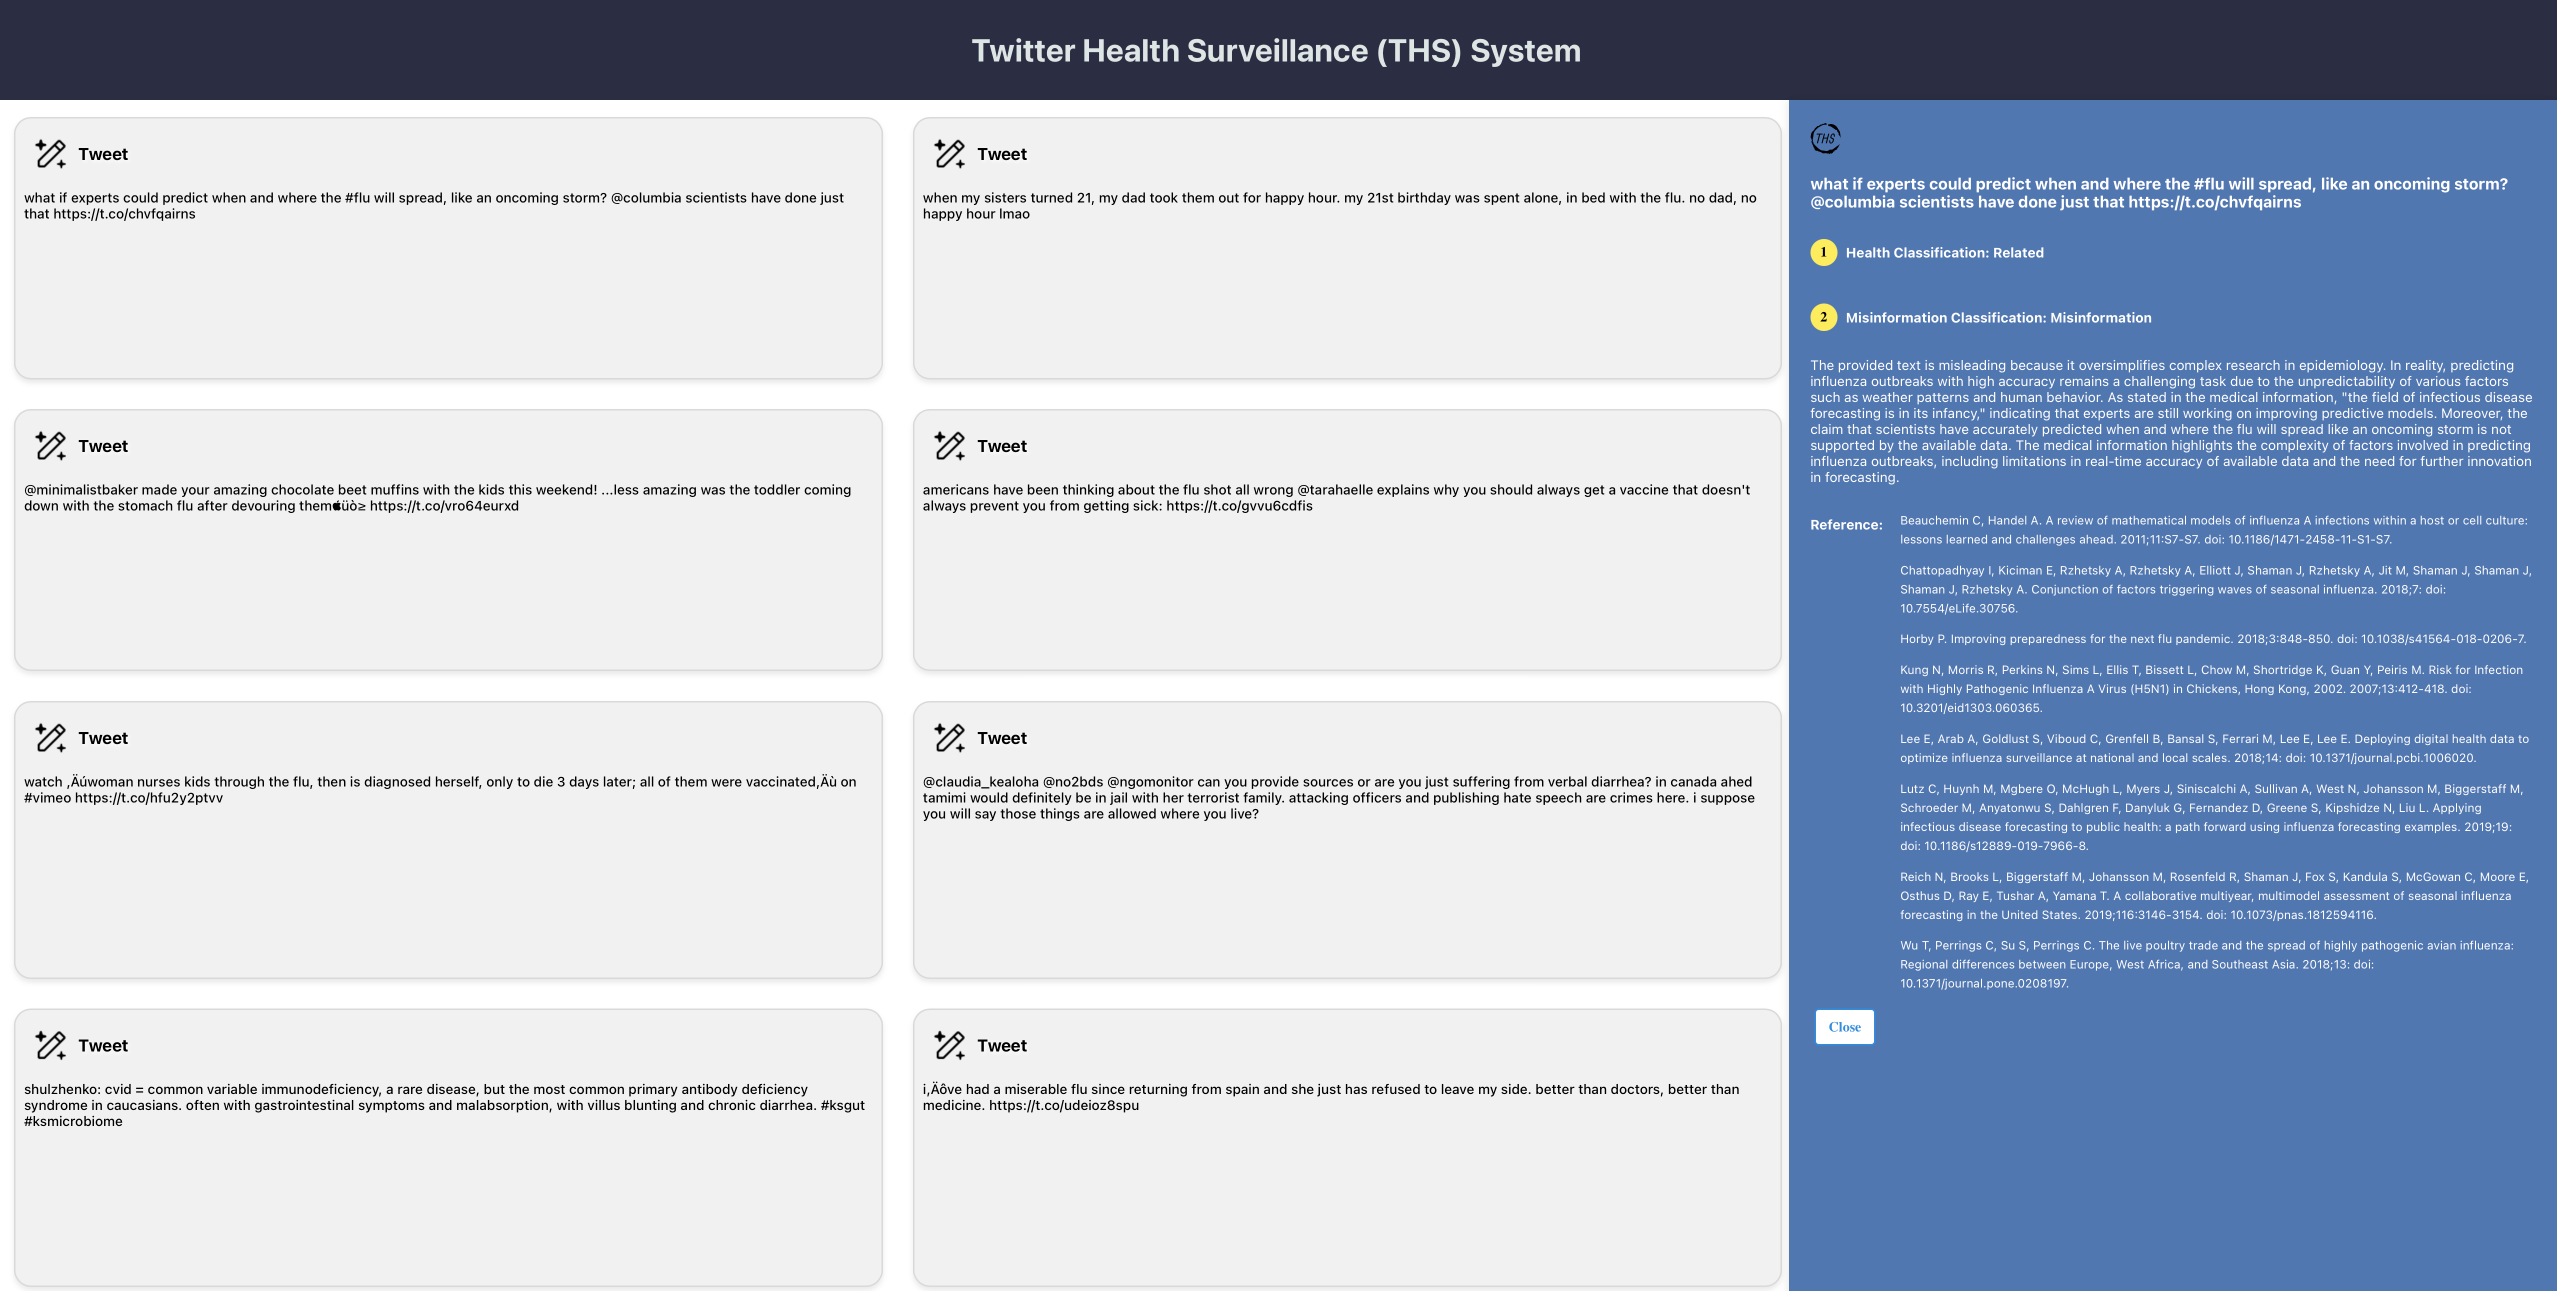
\includegraphics[width=0.75\paperwidth]{images/THS_Misleading.png} %specify width
	}%
	\caption{THS Frontend - Misinformation Classification } %specify caption
	\label{fig:frontendmisinformation}
\end{figure}


\begin{figure}[H]
\noindent\makebox[\textwidth][l] {%
	\hspace{-\dimexpr\oddsidemargin}
		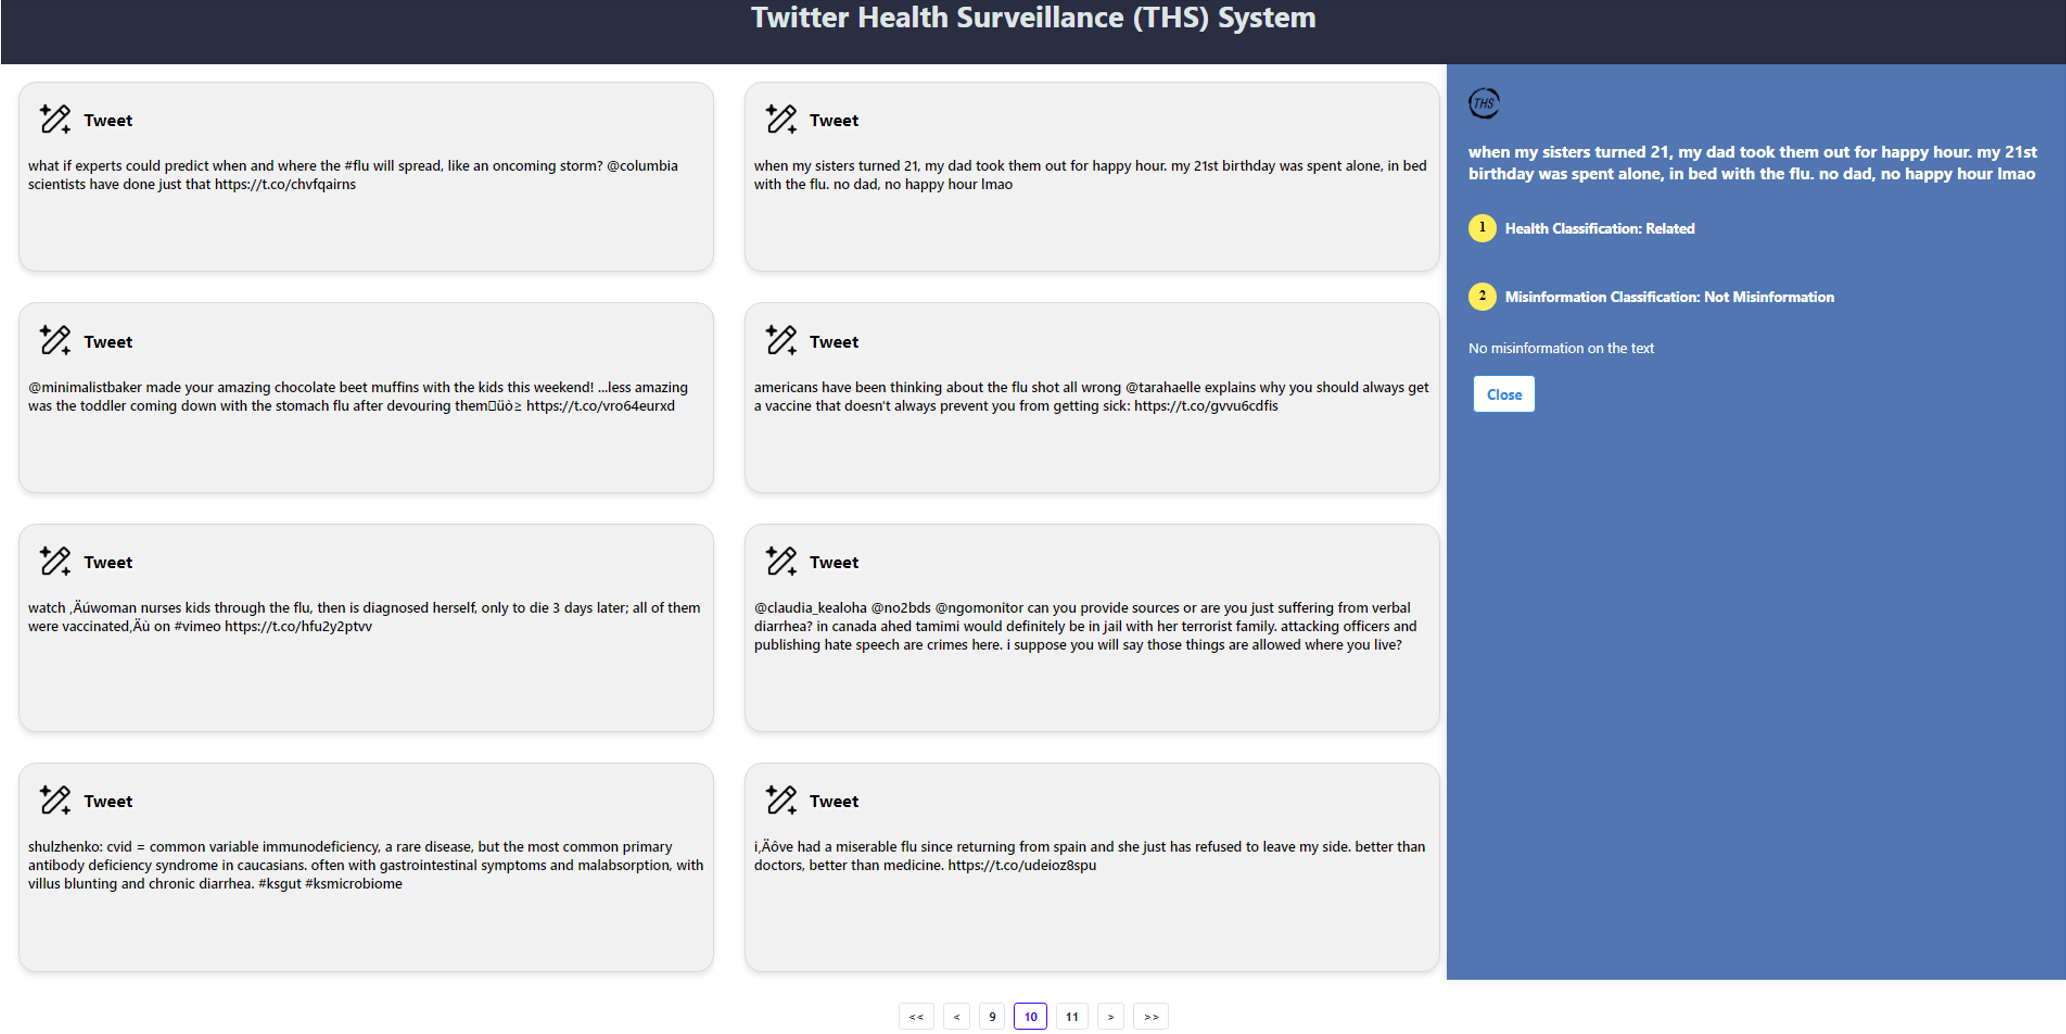
\includegraphics[width=0.75\paperwidth]{images/THS_NotMisinformation.png} %specify width
	}%
	\caption{THS Frontend  - No Misinformation Classification} %specify caption
	\label{fig:frontendnonmisinformation}
\end{figure}




% Define a custom style for JSON formatting
\lstdefinelanguage{json}{
    basicstyle=\ttfamily\small,
    numbers=left,
    numberstyle=\tiny\color{gray},
    stepnumber=1,
    numbersep=8pt,
    showstringspaces=false,
    breaklines=true,
    frame=single,
    backgroundcolor=\color{gray!10},
    keywordstyle=\color{blue},
    stringstyle=\color{red},
    morestring=[b]",
    morecomment=[l]{:}
}




\chapter{System Architecture}  

\section{Paper ETL Pipeline}

Our model must use credible sources of information to rebut misinformation. We identified PubMed \textbf{[REFERENCES]}, an online library that contains peer-reviewed medical literature. We want to extract the papers and store them in a vector database. To extract these papers, we used the BioC API \cite{bioinformatics}, which has access to the PubMed library. However, the API needs the research paper's identifier, known as PubMed Central (PMC) ID. We design a scraper to extract these identifiers from the official PubMed site. The pipeline in Figure \ref{fig:etl} shows the processes of data extraction. 

\subsection{Scraper}
The first step of the pipeline was identifying what papers we needed to extract. We selected 17 topics for the data extraction process. These topics are:

\begin{figure}[!ht]
	\begin{center}
		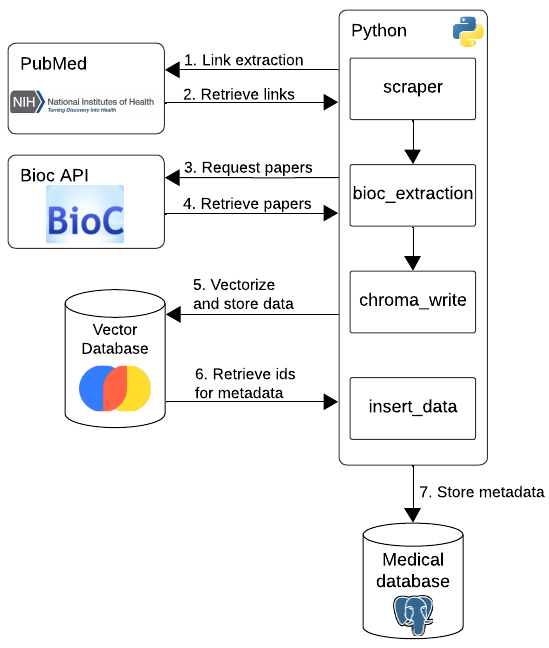
\includegraphics[width=0.75\textwidth]{images/ETL_Pipeline.png} %specify width
	\end{center}
	\caption{Medical Data Extraction Pipeline} %specify caption
	\label{fig:etl}
\end{figure}

\begin{multicols}{2}
	\begin{itemize}[topsep=0pt, partopsep=0pt, parsep=0pt]
	
	\item{allergy}
	\item{bird flu}
	\item{cancer}
	\item{chickenpox}
	\item{common cold}
	\item{conjunctivitis}
	\item{covid sickness}
	\item{covid symptoms}
	\item{covid treatment}
	\item{covid vaccine}
	\item{flu vaccine}
	\item{headache}
	\item{influenza}
	\item{monkeypox}
	\item{stomach aches}
	\item{swine flu}
	\item{zika}

	\end{itemize}

\end{multicols}



To extract them, we built a scraper in Python using Selenium and BeautifulSoup libraries. We used Selenium to retrieve the web source from PubMed's website, and BeautifulSoup was used to get the links to each paper. These links contained the PMC identifier. For each topic, we selected 5,000 PMC identifiers. These identifiers were grouped by topic and stored locally in Comma Separated Value (CSV) files.

\subsection{BioC API}
After retrieving those identifiers, we need to extract the research papers. Using the PubMed API, BioC, we made requests that returned the documents as JSON. These JSONs were preprocessed to contain texts, and we removed tables and figures. Later, the paper's sections -introduction, methodology, results, and others- were combined as one attribute, excluding references. We removed tables, figures, and references from the context to ensure the chunking process worked appropriately. If the data is not preprocessed, when performing RAG, we can retrieve data that is not useful. After that, we turned the result into a new JSON that contained the research metadata and its context. 

\subsection{Vectorizing data}
Later, each research paper’s context was split into chunks using LangChain. Then, we used an LLM, BAAI \cite{bge_embedding}, to embed these chunks. A universal unique identifier (UUID) was combined with each chunk and stored in a Chroma \cite{chroma} database. After uploading the data to Chroma, we added these UUIDs to their JSON. 


\subsection{Store metadata}
Now, with all papers vectorized, we upload the metadata into a Postgres database. First, we validate that there are no duplicate records in the system. To prevent duplicates, we search for the paper's reference. If any is found, we delete the chunks from the vector database. Additionally, any research that did not contain at least an abstract was removed. That ensures that there is no repetition or inconsistency when doing the rebuttal. Later, we upload this data into the system following the schema found in Figure \ref{fig:table}. The tables in this schema are as follow:

\begin{description}
	\item{\textbf{Research:}}  The table contains the research paper data. Its attributes are title, which is the research paper title; context, the paper’s text; paper\_ref, the complete reference of the paper, used to prevent duplicates; and fullpaper, which is a boolean that is true if the paper contains an abstract, introduction, methodology, discussion, conclusion, and references.
	\item{\textbf{Chunks:}} This table pairs the UUIDs from the paper's chunks and their respective research record.  
	\item{\textbf{Keyword:}} Some research papers contain keywords that allow the reader to know the subjects mentioned in the paper. 
	\item{\textbf{Author:}} Stores the first and last names of all authors identified in the research paper. 
	\item{\textbf{Reference:}} All references that are present in the research paper.
	\item{\textbf{Topic:}} This contains the different topics used to search the papers.

\end{description}

\begin{figure}[H]
	\begin{center}
		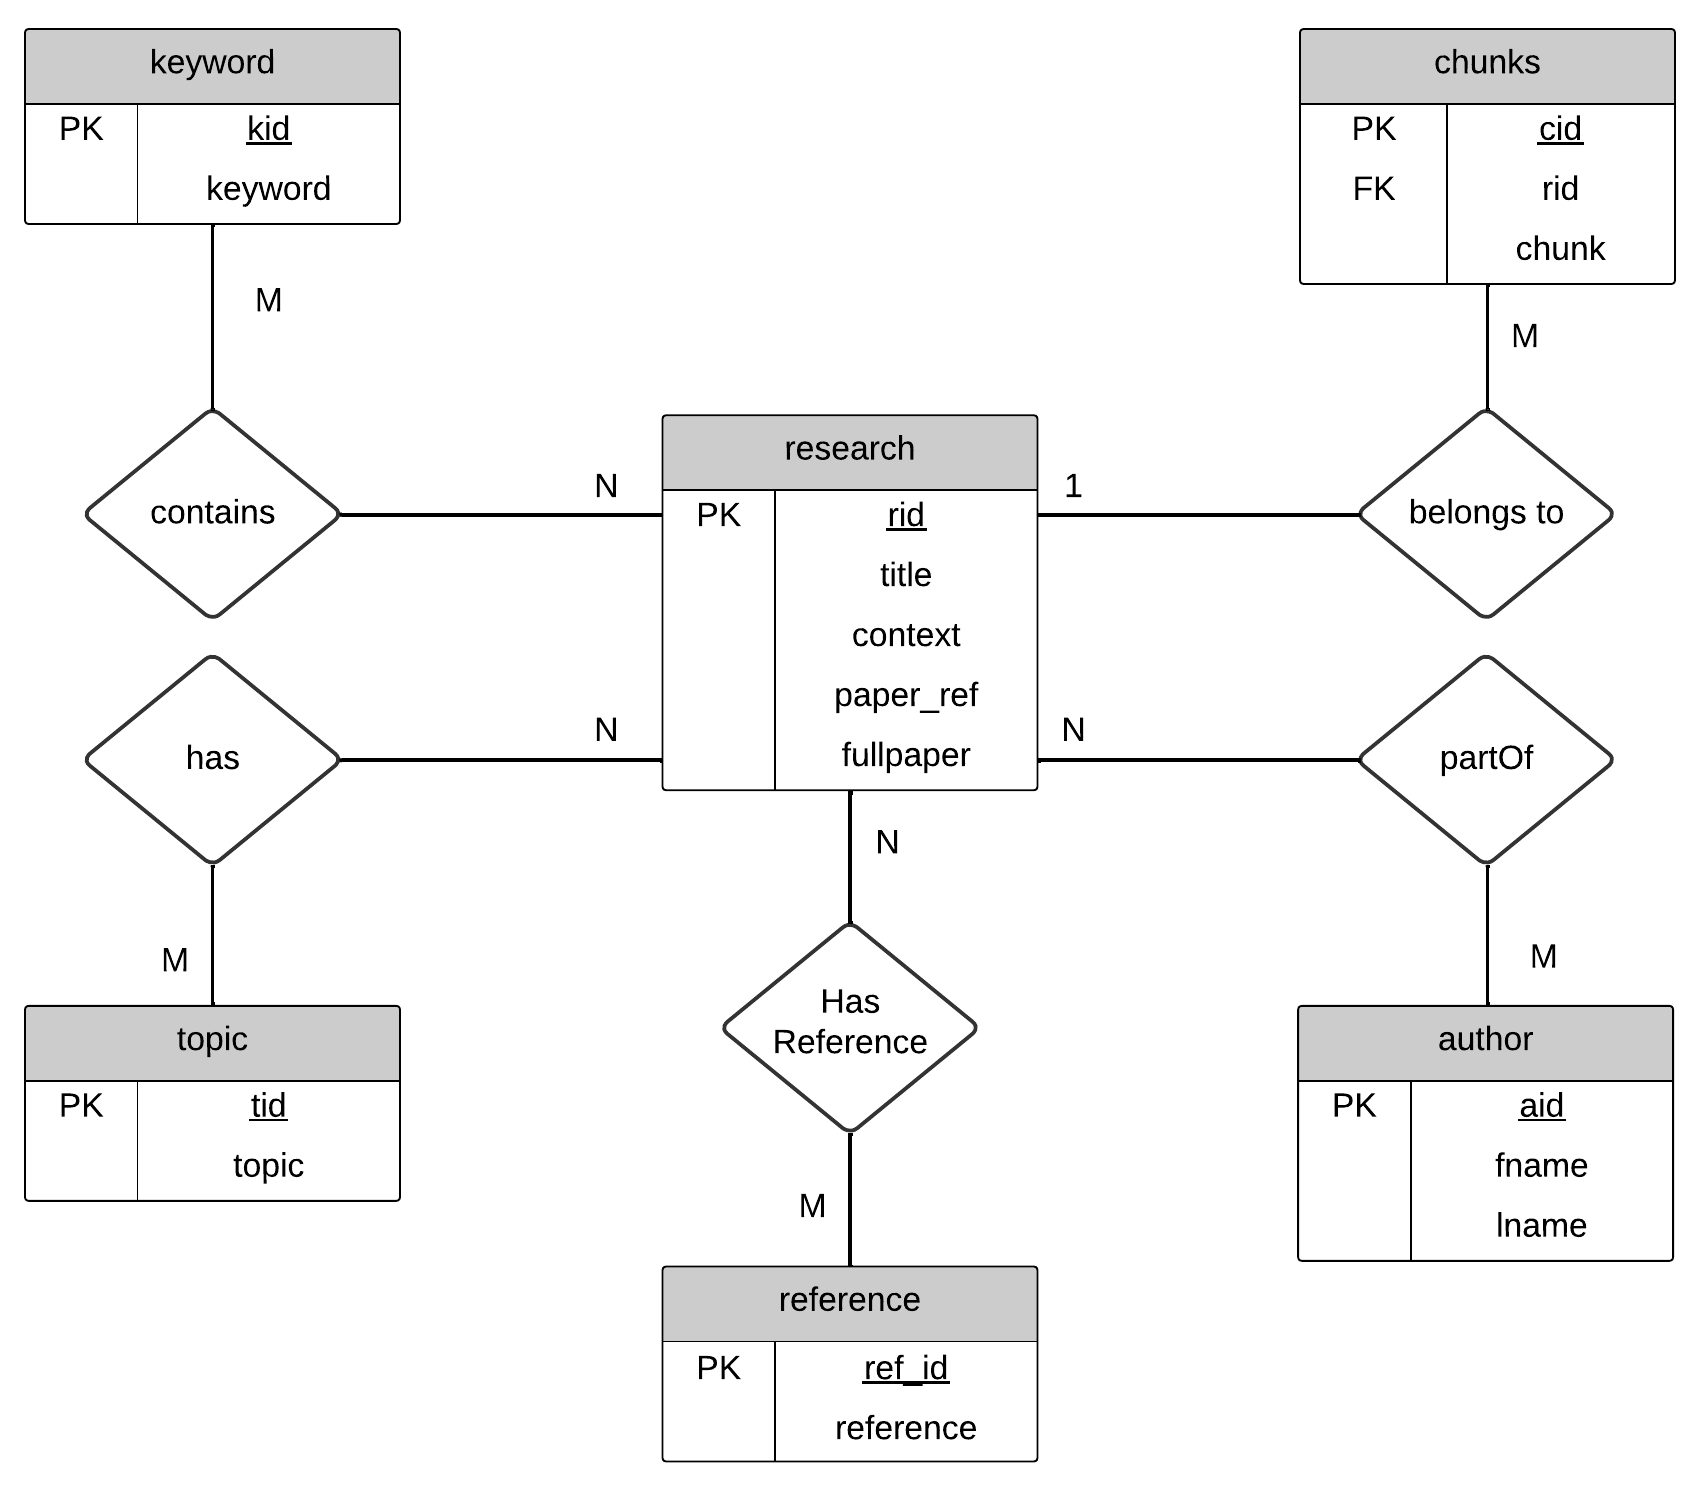
\includegraphics[width=0.9\textwidth]{images/Table_diagram.png} %specify width
	\end{center}
	\caption{Research Papers Schema Diagram} %specify caption
	\label{fig:table}
\end{figure}


We started the search with 85,000 peer-reviewed papers. After finishing the filtering and data cleaning, we ended with 56,365 different research papers. 



\section{Misinformation Rebuttal Pipeline}
After training the models and storing the context for the rebuttal, we create the model pipeline. The pipeline shown in Figure \ref{fig:llm} shows the process of receiving a text, making the classifications, and returning an explanation of why it is misinformation.

\begin{figure}[H]
	\begin{center}
		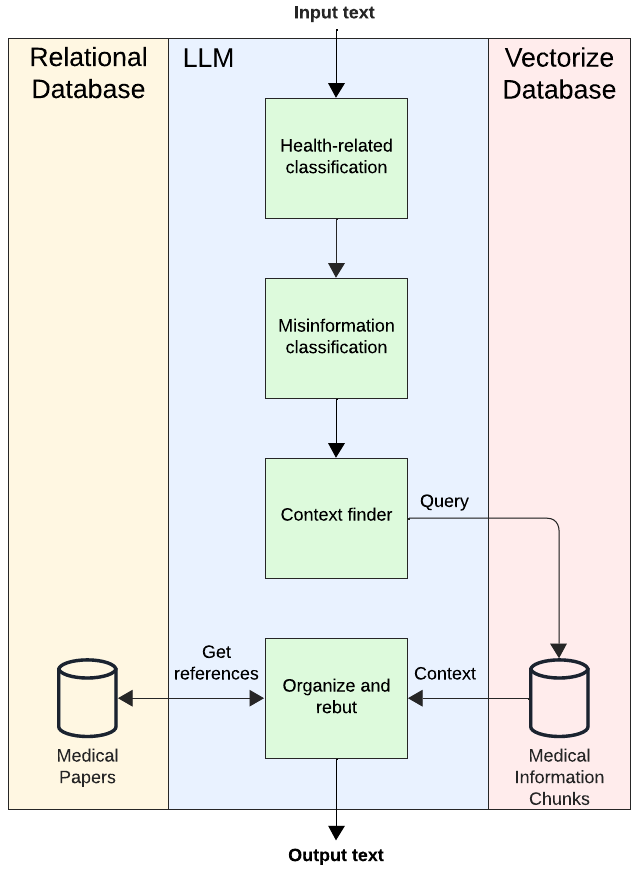
\includegraphics[width=0.75\textwidth]{images/LLM_Pipeline} %specify width
	\end{center}
	\caption{Misinformation Rebuttal LLM System Architecture} %specify caption
	\label{fig:llm}
\end{figure}


\subsection{Health-related Classification}
The first part of the pipeline is determining if the text is related to health. When the system receives the input text, it sends it to a model finetuned to classify health-related texts. This model determines whether the input is related, unrelated, or ambiguous.
If the text is health-related, we continue to the next part of the pipeline. When the text is non-related or ambiguous, we end the process. We end this because other topics are out of the model's scope. 

\subsection{Misinformation Classification}
After confirming that the text is health-related, we want to validate that it contains misinformation. The finetuned model can only return two possible results: misinformation or non-misinformation. If the model finds no misinformation after evaluating the text,
the final output will return both classifications. When the result contains misinformation, we start the search for research papers.

\subsection{Context Finder}
Before starting the search on the vector database, we must understand the topic of the text. To understand the text, we send a query to Ollama asking it to make a one-sentence query for the vector database related to the input.

%\noindent \textbf{Example} Tweet: "\textit{\#nih fauci, @cdcdirector @sgottliebfda \&amp; @barda bright expected to be grilled tomorrow over ineffective \#flu vaccine at @housecommerce \#suboversight  bets on fauci saying universal \#influenza vax in 5, maybe 10 years? my preview here: https://t.co/fsqefwhik7  \#cdc \#fda \#vaccines}"
%Ollama output: "\textit{What are the implications of the House Commerce Suboversight Committee questioning NIAID Director Fauci and other officials about the efficacy of flu vaccines, particularly regarding universal influenza vaccination in the next 5-10 years?}"
 
 \begin{tcolorbox}[colback=gray!10, colframe=black!70, title=Input]
\texttt{%
\#nih fauci, @cdcdirector @sgottliebfda \&amp; @barda bright expected to be grilled tomorrow over ineffective \#flu vaccine at @housecommerce \#suboversight bets on fauci saying universal \#influenza vax in 5, maybe 10 years? my preview here: \url{https://t.co/fsqefwhik7} \#cdc \#fda \#vaccines%
}
\end{tcolorbox}

\begin{tcolorbox}[colback=white, colframe=black!70, title=Output]
\textit{%
Flu vaccine effectiveness and future universal influenza vaccination strategies.%
}
\end{tcolorbox}
 
The above example shows that Ollama can identify the topics of the original text. That tweet mentions that the flu vaccine is ineffective and asks how long it will take for a universal influenza vaccine. The LLM identified the topic and made a query that can help find
research papers related to it. However, it is essential to mention that the LLM output can vary. As mentioned previously, this is a statistical model and can have slight variations in its result. Now, this output is sent to the Chroma database to retrieve chunks of research
papers. For this experiment, our model returns eight chunks that are closest in context to the query. These chunks are then sent to another model to be analyzed and organized.

\subsection{Organize and Rebut}
The final part of our pipeline is using RAG to provide an answer that explains why the original text is misinformation. First, we retrieve the references of the chunks we use for the context. Then, we send the original text with the chunks, as context, to Ollama for
the model to evaluate. Ollama returns a 2-3 sentence result that explains the text’s misinformation. The final output is a JSON with the following attributes:

\begin{description}
\item{\textbf{chroma\_value:}} If the text is health-related and is misinformation, this will have the rebuttal output from Ollama, consisting of 2-3 sentences. If the text is non-related or non-misinformation, it will give a default value saying so. 
\item{\textbf{health:}} This is the input text health classification.
\item{\textbf{misinformation:}} This is the input text misinformation classification.
\item{\textbf{references:}} This attribute stores the list of references used for the rebuttal. 
\item{\textbf{t\_context:}} The original text.

\end{description}

The pipeline enables us to automate the classification process and rebut misinformation using peer-reviewed research. By leveraging fine-tuned models, vector search, and RAG, the architecture provides concise, fact-based responses. A key advantage of this
approach is its ability to explain complex content accessible to non-technical readers, giving them a clearer understanding of false information. This can assist professionals in the field to mitigate the spread of lies that can negatively impact public health.

%\begin{lstlisting}[language=json]
%{
%  "chroma_value": "The text claims that the current flu vaccine is ineffective and implies a specific timeline for developing a universal influenza vaccine. However, researchers are still working on overcoming the limitations of current influenza vaccines, ...",
%  "health": "Related",
%  "misinformation": "Misinformation",
%  "references": "[Choi A, Garcia-Sastre A, Schotsaert M. Host immune response-inspired development of the influenza vaccine.  2020;125:28-35. doi: 10.1016/j.anai.2020.04.008., ... ]",
%  "t_context": "#nih fauci, @cdcdirector @sgottliebfda &amp; @barda bright expected ...",
%}
%\end{lstlisting}



%\begin{enumerate}
	%\item Health-related classification: Verifies if the inputted text is health-related. The possible options are related, unrelated, or ambiguous.
	%\item Misinformation classification: If the text was classified as health-related, we then checks if the text contains misinformation. If any misinformation is detected, we need to find official health data to rebut said misinformation.
	%\item	Context finder: A query is created for a vector database based on the original text. This query is sent to a vectorized database, Chroma, and will return chunks that are related to the query.
	%\item	Medical information database:  This is a database that contains medical metadata from official sources. Using the chunk IDs we will retrieve the original papers' references.
	%\item	Organize and rebut: The result from the medical database is now processed and used to make a rebuttal for the misinformation in the text. Then, we query the relational database to extract the references of the papers used for the previous part.
	%The output includes the original text, the health and misinformation classifications, the correction of the misinformation, and the citation of the sources used. 
%\end{enumerate}













\chapter{Performance Evaluation}  
This section presents the results of our models on the classification tasks. The results show each model's precision, recall, f1 score, and training time.


\section{Health-Related Classification}
We present the results of the health classification process and compare them with the best overall model of the previous THS project. They concluded
that their best model is an LSTM, with no attention, and a GRU layer.

\subsection{Precision}
\begin{table}[H]
	\centering
	\caption{Health Related Precision Result}
	\begin{tabular}{||c | c||} 
		\hline
		\textbf{Model} & \textbf{Result} \\ [0.5ex] 
		\hline
		BERT & 0.85  \\
		\hline
		LLaMa-2 & 0.94 \\ 
		\hline
		LSTM GRU NO ATTENTION & 0.83  \\
		\hline
		T5 (Causal) & 0.85 \\
		\hline
		T5 (Sequence) & 0.48 \\
		\hline
	\end{tabular}
	\label{table:HealthPrecision}
\end{table}

Table \ref{table:HealthPrecision} shows the result for the precision metric for the related classification. For clarity, we focus on this class because our project
goal is to detect health-related misinformation. The best-performing model here was the LLaMa-2 model, which has a precision of 94\%. Tied for second place
are BERT and T5 (Causal), with 85\% precision. Next is the THS model, with 83\% precision. Lastly, we have a T5 (Sequence) model with a relatively low
precision of 48\%.

\subsection{Recall}
\begin{table}[H]
	\centering
	\caption{Health Related Recall Result}
	\begin{tabular}{||c | c||} 
		\hline
		\textbf{Model} & \textbf{Result} \\ [0.5ex] 
		\hline
		BERT & 0.91  \\
		\hline
		LLaMa-2 & 0.84 \\ 
		\hline
		LSTM GRU NO ATTENTION & 0.89  \\
		\hline
		T5 (Causal) & 0.95 \\
		\hline
		T5 (Sequence) & 0.44 \\
		\hline
	\end{tabular}
	\label{table:HealthRecall}
\end{table}

Table \ref{table:HealthRecall} shows the result for the recall metric for the related classification. When comparing this metric with the THS investigation, there is a noticeable difference. Their results
show that only the LSTM layer, no attention, and a GRU layer model was the only one with a result over 80\%. In contrast, most of our models had a score of at least 80\%. Comparing this result
with the precision table (Table \ref{table:HealthPrecision}, our model did not score drastically lower. Here, our best model was T5 (Causal), with a performance of 95\% in recall. Next, we have
BERT with 91\%, followed by the THS model with 89\%. Then, the model with the highest precision, LLaMa-2, ended with 84\%. Lastly, we have again the T5 (Sequence) model with a 44\%,
lower than its precision.

\subsection{F1}
\begin{table}[H]
	\centering
	\caption{Health Related F1 Result}
	\begin{tabular}{||c | c||} 
		\hline
		\textbf{Model} & \textbf{Result} \\ [0.5ex] 
		\hline
		BERT & 0.88  \\
		\hline
		LLaMa-2 & 0.89 \\ 
		\hline
		LSTM GRU NO ATTENTION & 0.86  \\
		\hline
		T5 (Causal) & 0.90 \\
		\hline
		T5 (Sequence) & 0.46 \\
		\hline
	\end{tabular}
	\label{table:HealthF1}
\end{table}

Table \ref{table:HealthF1} shows the result for the F1 metric for the related classification. The F1 score is the balance between precision and recall. When we compare the results with the
THS model, most models have a higher F1 score. The results show that T5 (Causal) had 90\%, LLaMa-2 with 89\%, BERT ended with 88\%, and T5 (Sequence) scored a 46\%. In contrast,
the THS model had an 86\%, ending in second to last place.

\subsection{Training Time}

In Figure \ref{fig:HealthTime}, we present our model's training time. As mentioned earlier, we trained each model for 20 epochs with a batch size of 16. BERT trained faster than
any other model, which took 187 minutes. The T5 (Sequence) model took 1442 minutes, while the T5 (Causal) model finished in 1569 minutes. Lastly, LLaMa-2 took 5126 minutes to
train. Based on these results, we can infer that models with fewer parameters train faster. BERT trained 27.4x faster than LLaMa-2.

\begin{figure}[H]
	\begin{center}
		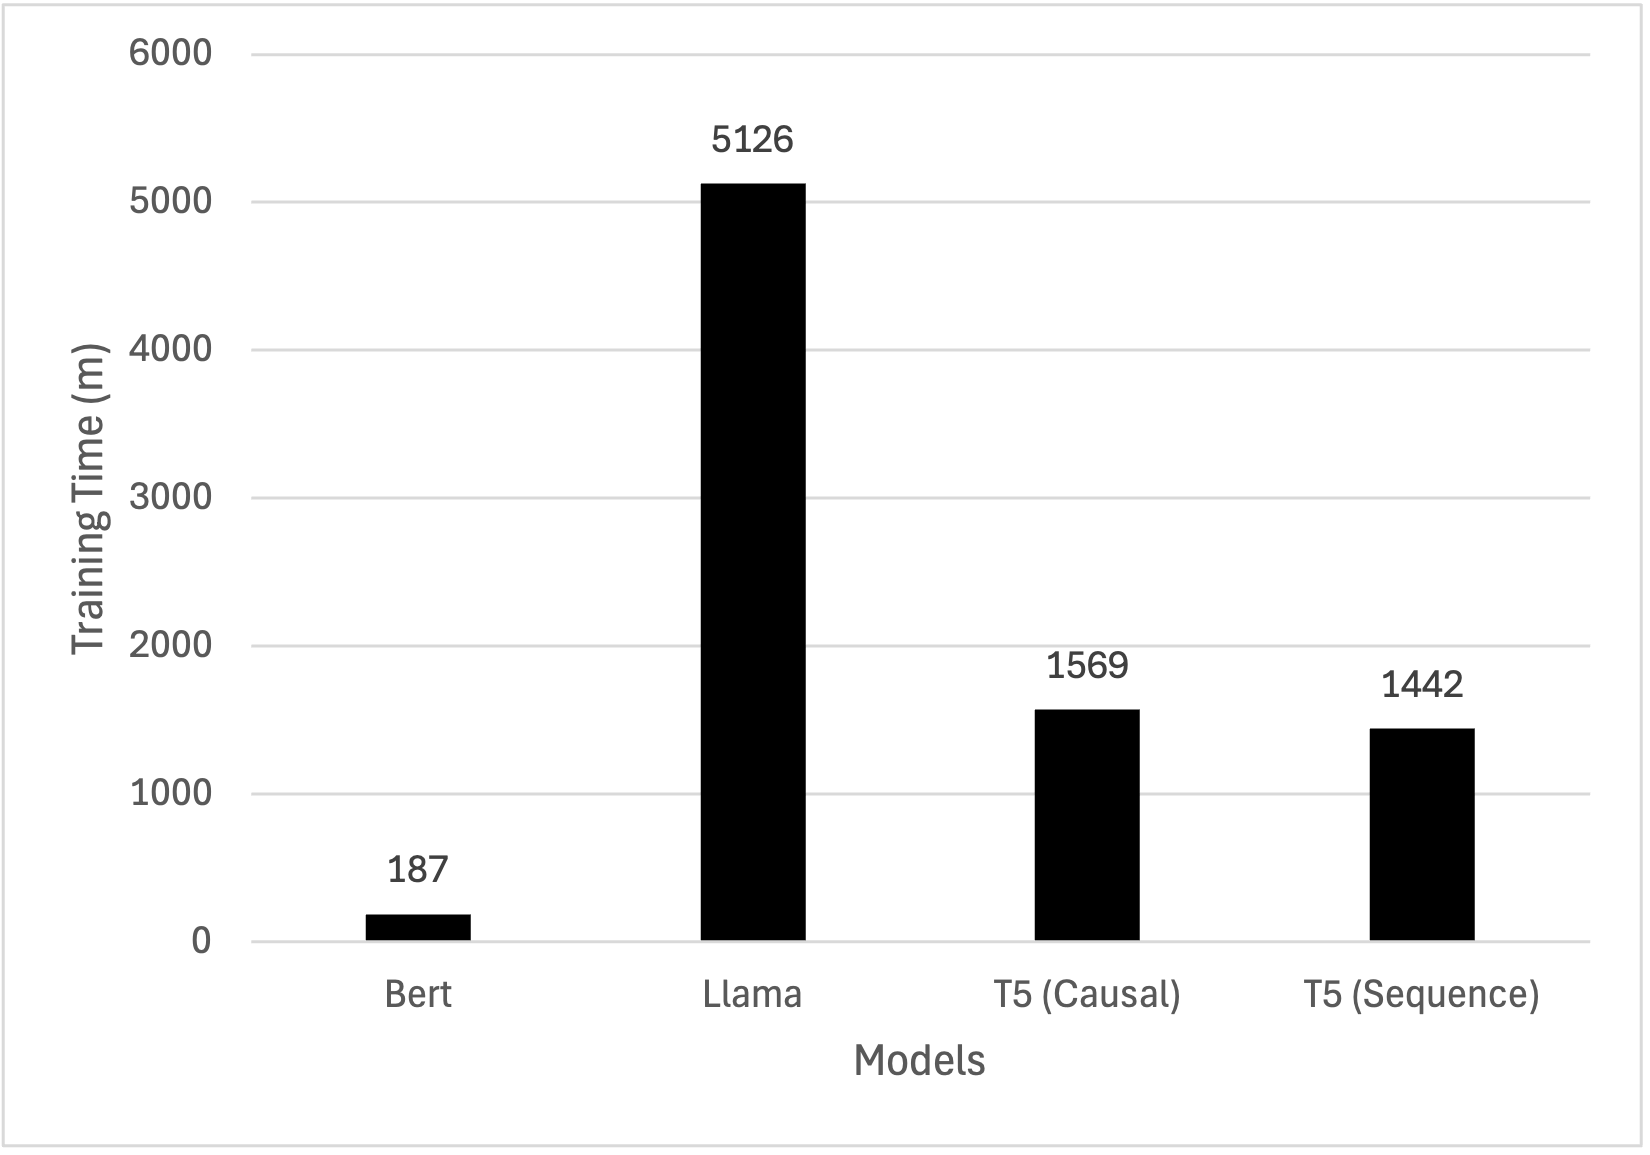
\includegraphics[width=1\textwidth]{images/Health_related_training_time.png} %specify width
	\end{center}
	\caption{Health-Related Models Training Time} %specify caption
	\label{fig:HealthTime}
\end{figure}


\section{Misinformation Classification}
In this section, we present the misinformation classification results. However, in this section, we did not compare with the THS model because they did not train a model to classify
misinformation.

\subsection{Precision}
\begin{table}[H]
	\centering
	\caption{Misinformation Precision Result}
	\begin{tabular}{||c | c||} 
		\hline
		\textbf{Model} & \textbf{Result} \\ [0.5ex] 
		\hline
		BERT & 0.90  \\
		\hline
		LLaMa-2 & 0.98 \\ 
		\hline
		T5 (Causal) & 0.99 \\
		\hline
		T5 (Sequence) & 0.99 \\
		\hline
	\end{tabular}
	\label{table:MisinformationPrecision}
\end{table}

Table \ref{table:MisinformationPrecision} shows the result for the precision metric for the misinformation classification. In this case, we focus on the misinformation
class because it is our project goal. Our best-performing models here were both T5 models, which have a precision of 99\%. The next model with the highest precision
was LLaMa-2, with a score of 98\% precision. The lowest-performing model was BERT, which resulted in 90\% precision. Nonetheless, all models had a score of at least 90\%.


\subsection{Recall}
\begin{table}[H]
	\centering
	\caption{Misinformation Recall Result}
	\begin{tabular}{||c | c||} 
		\hline
		\textbf{Model} & \textbf{Result} \\ [0.5ex] 
		\hline
		BERT & 0.94  \\
		\hline
		LLaMa-2 & 0.95 \\ 
		\hline
		T5 (Causal) & 0.92 \\
		\hline
		T5 (Sequence) & 0.85 \\
		\hline
	\end{tabular}
	\label{table:MisinformationRecall}
\end{table}

Table \ref{table:MisinformationRecall} shows the recall metric's results for the misinformation classification. When we compare these results with the precision table 
(Table \ref{table:MisinformationPrecision}), our model maintains a similar score. Here, the model with the best results was LLaMa-2, with a performance of 95\%.
Next, we have BERT with 94\% and T5 (Causal) with a 92\% recall. Finally, T5 (Sequence) ended with 85\% in the recall.


\subsection{F1}
\begin{table}[H]
	\centering
	\caption{Misinformation F1 Result}
	\begin{tabular}{||c | c||} 
		\hline
		\textbf{Model} & \textbf{Result} \\ [0.5ex] 
		\hline
		BERT & 0.92  \\
		\hline
		LLaMa-2 & 0.97 \\ 
		\hline
		T5 (Causal) & 0.96 \\
		\hline
		T5 (Sequence) & 0.92 \\
		\hline
	\end{tabular}
	\label{table:MisinformationF1}
\end{table}


Table \ref{table:MisinformationF1}  shows the result for the F1 metric for the misinformation classification. This result balances precision and recall. The results show that the model
with the best F1 was LLaMa-2 with a 97\%. Next is T5 (Causal) with a 96\% F1, and tied to last, we have BERT and T5 (Sequence) with 92\%. All models had an optimal F1 score over 90\%.


\subsection{Training Time}

In Figure \ref{fig:MisinformationTime}, we present the training time for the misinformation models. We trained the models using the same parameters as in the Health-Related classification.
When we compare these results with the Health-Related (Figure \ref{fig:HealthTime}), the average training time was less. A possible reason is that we used less data for the training. The
only exception was BERT, which took 351 minutes to train. Next is T5 (Causal) with 371 minutes and T5 (Sequence) with 1274 minutes. Finally, LLaMa-2 took 2840 minutes to train. A noticeable difference was T5 (Causal), which trained 4.23x faster for this dataset compared to the health-related dataset. Nonetheless, BERT finished the fastest, being 8.10x faster than LLaMa-2.


\begin{figure}[H]
	\begin{center}
		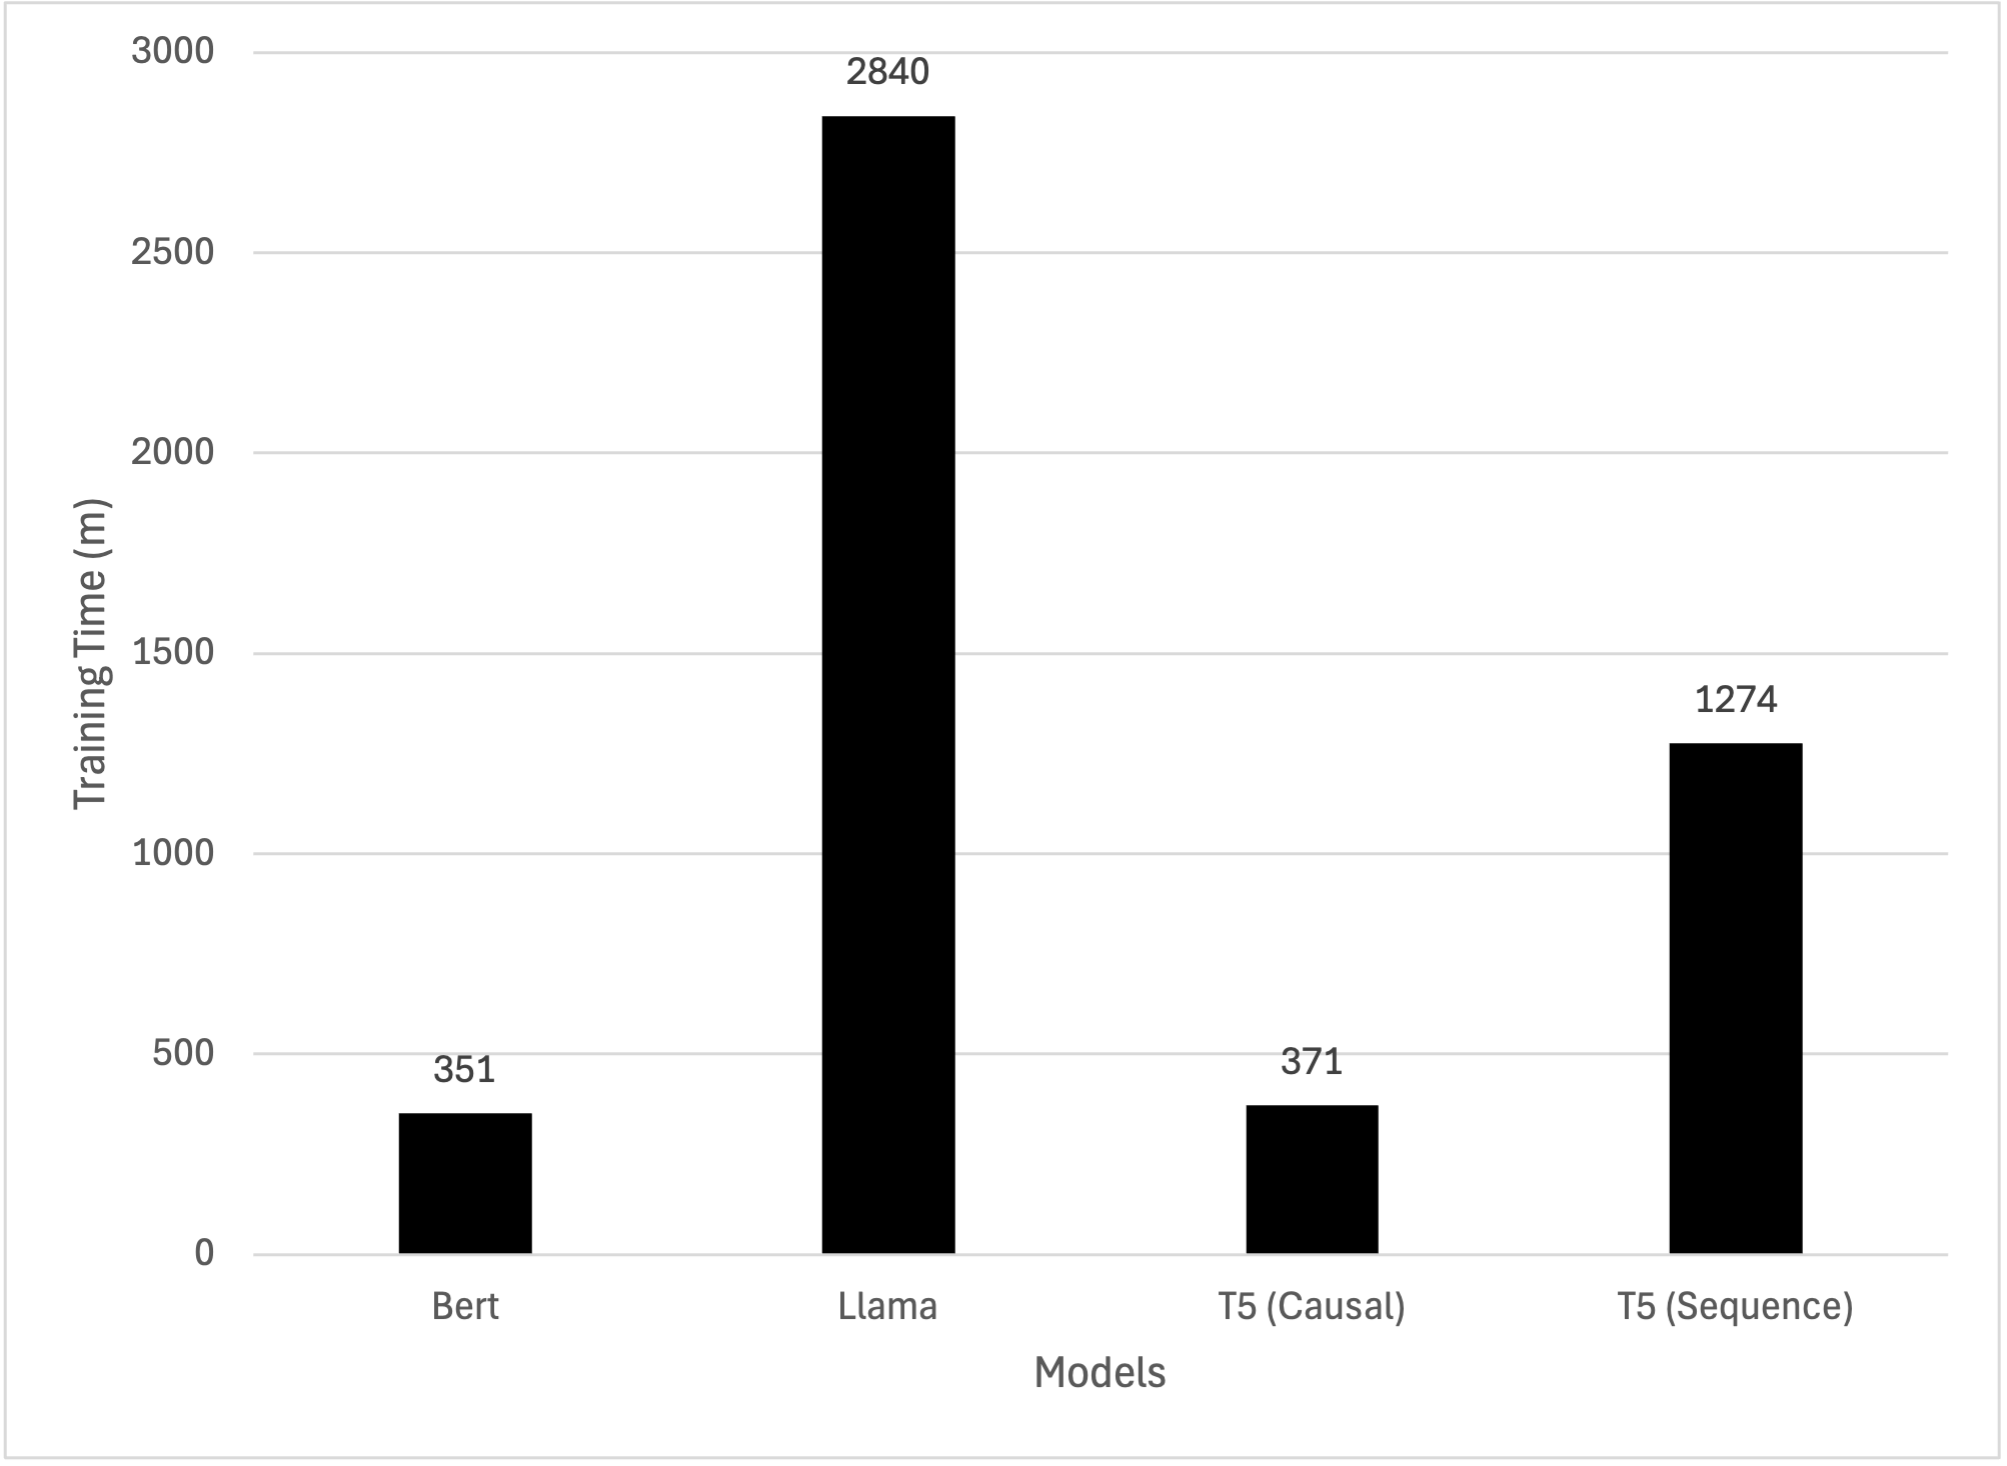
\includegraphics[width=1\textwidth]{images/Misinformation_training_time.png} %specify width
	\end{center}
	\caption{Misinformation Models Training Time} %specify caption
	\label{fig:MisinformationTime}
\end{figure}



\section{Discussion}

The results present that most LLMs outperformed the THS model. We applied preprocessing techniques such as replacing links, mentions, and hashtags with special tokens. The training
parameters for all models were 20 epochs, batch size of 16, 8bit initialization, and adamw\_8bit optimizer. Additionally, the LoRA hyperparameters were 16 for the rank, an alpha of 32, a dropout
of 0.05, and a bias for all parameters. The score metrics we used for the model evaluation were precision, recall, and F1. In our case, we want to focus on F1. That metric helps us reduce false
negative results but not overclassify false positives.

Our model with the best result for the health-related classification (Table \ref{table:HealthF1}) was T5 (Causal), with a 90\% F1 score, while the THS model had 86\%. However, the trade-off
for this model is that the training is computationally expensive. The reason is that labels in T5 (Causal) are text instead of numbers. Those texts must be embedded, which requires more
processing power. Also, that model cannot have class weights because of the structure of the embedding. Additionally, the training time  (Figure \ref{fig:HealthTime}) for T5 is more extensive
when compared to BERT, 8.4x. Now, BERT had a slightly lower result with 88\%. Nonetheless, when we factor in the training time and processing power, this model is more efficient.

The model with the highest F1 score for the misinformation classification (Table \ref{table:MisinformationF1}) was LLaMa-2, followed by T5 (Causal), 97\% and 96\%, respectively. These two models
have desirable results for this classification task. However, both require high computational power, and LLaMa-2 has an extensive training time (Figure \ref{fig:MisinformationTime}) compared to BERT,
8.09x more. It is important to notice that in both scenarios, LlaMa-2 and T5 (Causal) outperform the other models by a slight margin. These models contain a Decoder element, which can help them
generate and understand text appropriately.

This project focuses on social media posts, and we know that there are frequent changes in how users interact. Additionally, when new diseases are found or named, we must retrain most
models to add these words to their vocabulary. Retraining can be costly if the model has many parameters and requires extensive training. Thus, we can say that BERT had overall results
that can help combat health misinformation on social media. That model had an F1 score of 88\% in health and 92\% in misinformation classification. Finally, that model took less overall time
to train and used the least amount of RAM.











%


\chapter{Methodology}  

\section{Section}
\noindent \lipsum[1][1-3] %WRITE HERE

\subsection{Subsection}
\noindent \lipsum[1][3-5] %WRITE HERE

\subsubsection{Subsubsection}
\noindent \blindtext %WRITE HERE

\subsection{Subsection}
\noindent \lipsum[1][2-5] %WRITE HERE






%

\chapter{Results}  

\section{Section}





\chapter{Conclusions \& Future Work}  

\section{Conclusions}
\noindent In this thesis, we presented how LLMs can be used to refute health misinformation in social media. Additionally, we demonstrated that certain elements within a text—such as mentions, hashtags, and links—play a significant role in shaping its meaning. We also presented how we extracted, processed, stored, and used research papers with LLMs for the misinformation rebuttal. Finally, the research shows that it is possible to fine-tune large models with limited memory using LoRA.

A prototype version of the misinformation rebuttal pipeline was implemented with Python, Postgres, Chroma, and other open-source tools. The research presents the performance results using health-related tweets and misinformation texts from different online sources. Our research preliminary performance results show that we can achieve an F1 score of 90\% for health-related classification and 97\% for misinformation classification. Additionally, we present that the model can refute misinformation by generating an answer using RAG. Thus, the project can help health experts combat misinformation and reduce the risk of negatively impacting public health.

\section{Future Work}

\begin{description}

\item{\textbf{Additional Models for Classification:}} It is possible to train alternative LLM  for the classification tasks.

\item{\textbf{Processing Time:}} During our experiment, we noticed that the misinformation pipeline takes excessive time to process. The processing time is mostly caused by the search in the vector database. Exploring different vector databases and similarity search algorithms can improve the processing time.

\item{\textbf{Rebuttal Helpfulness:}} The rebuttal the model generates must be as useful as possible for non-technical readers. That rebuttal can include specific information about the disease, such as symptoms, treatment, statistics, and other relevant factors.

\end{description}
\bibliography{referencias} 
\addcontentsline{toc}{chapter}{References}
\newpage


%%______________APPENDICES CONTENT______________________________
%% _____________APPENDIX A______________________________________
%\addcontentsline{exp}{chapter}{Appendix A: MATLAB Code} %Change title of Appendix A for List of Appendices
%%\example{MATLAB CODE}
%%\label{1st_ex}
%\chapter*{Appendix A: MATLAB Code} %Change title of Appendix A
%
%\noindent \lipsum[1][1-20] %WRITE HERE
%\noindent \lipsum[1][1-20] %WRITE HERE
%\noindent \lipsum[1][1-20] %WRITE HERE
%
%
%\newpage
%
%% _____________APPENDIX B______________________________________
%\addcontentsline{exp}{chapter}{Appendix B: Data} %Change title of Appendix B for List of Appendices
%\chapter*{Appendix B: Data} %Change title of Appendix B
%%\example{DATA}
%%\label{2nd_ex}
%\noindent \lipsum[1][1-3] %WRITE HERE
%
%\newpage
%
%% _____________APPENDIX C______________________________________
%\addcontentsline{exp}{chapter}{Appendix C: More Data} %Change title of Appendix C for List of Appendices
%\chapter*{Appendix C: More Data} %Change title of Appendix C
%%\example{DATA}
%%\label{2nd_ex}
%\noindent \lipsum[1][1-3] %WRITE HERE
%
%
%% _____________APPENDIX D______________________________________
%\addcontentsline{exp}{chapter}{Appendix D: More Data} %Change title of Appendix D for List of Appendices
%\chapter*{Appendix D: More Data} %Change title of Appendix C
%%\example{DATA}
%%\label{2nd_ex}
%\noindent \lipsum[1][1-3] %WRITE HERE

\end{document}